\begin{figure}

\centering

\begin{subfigure}[b]{0.45\textwidth}
\tikzsetnextfilename{Huu}

\centering
\resizebox{1\textwidth}{!}{
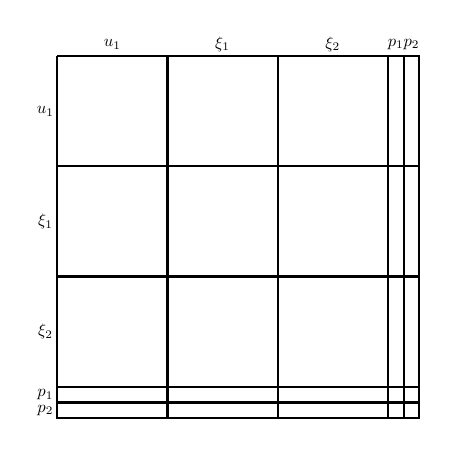
\begin{tikzpicture}[yscale=-1] 

\pgfmathsetmacro{\nt}{7};% time points
\pgfmathsetmacro{\nu}{1}; % controls
\pgfmathsetmacro{\nx}{2}; % states
\pgfmathsetmacro{\np}{2}; % parameters
\pgfmathsetmacro{\nc}{\nu + \nx}; % total continuous

%% control labels
\foreach \k in {1,...,\nu}{
	\pgfmathsetmacro{\x}{0.2*\nt*\k - 0.2/2*(\nt-1)};
	\node () at (\x,-0.05) {\scalebox{0.6}{$u_{\k}$}};
    \node () at (-0.05,\x) {\scalebox{0.6}{$u_{\k}$}};
}

%% state labels
\foreach \k in {1,...,\nx}{
	\pgfmathsetmacro{\x}{0.2*\nt*\k + 0.2*\nu*\nt - 0.2/2*(\nt-1)};
	\node () at (\x,-0.05) {\scalebox{0.6}{$\xi_{\k}$}};
    \node () at (-0.05,\x) {\scalebox{0.6}{$\xi_{\k}$}};
}

%% parameter labels
\foreach \k in {1,...,\np}{
	\pgfmathsetmacro{\x}{0.2*\k + 0.2*\nu*\nt + 0.2*\nx*\nt};
	\node () at (\x,-0.05) {\scalebox{0.6}{$p_{\k}$}};
    \node () at (-0.05,\x) {\scalebox{0.6}{$p_{\k}$}};
}


%% controls
\foreach \k in {1,...,\nu}{
	\foreach \j in {1,...,\nu}{
		\foreach \i in {1,...,\nt}{ 
        	\pgfmathsetmacro{\kk}{\k-1};
            \pgfmathsetmacro{\jj}{\j-1};
        	\pgfmathsetmacro{\x}{0.2*\i + 0.2*\kk*\nt};
            \pgfmathsetmacro{\y}{0.2*\i + 0.2*\jj*\nt};
        	\node () at (\x,\y) {\mysparsesymbol};
} 
    \pgfmathsetmacro{\kk}{\k-1};
    \pgfmathsetmacro{\jj}{\j-1};
    \pgfmathsetmacro{\x}{0.2*\kk*\nt + 0.1};
    \pgfmathsetmacro{\y}{0.2*\jj*\nt + 0.1};
	\draw[\mysparseboxcolor,thick](\x,\y) -- (\x+0.2*\nt,\y) -- (\x+0.2*\nt,\y+0.2*\nt) -- (\x,\y+0.2*\nt) -- (\x,\y);
} }

%% states
\foreach \k in {1,...,\nx}{
	\foreach \j in {1,...,\nx}{
		\foreach \i in {1,...,\nt}{ 
        	\pgfmathsetmacro{\kk}{\k-1};
            \pgfmathsetmacro{\jj}{\j-1};
        	\node () at (0.2*\i + 0.2*\kk*\nt + 0.2*\nu*\nt, 0.2*\i + 0.2*\jj*\nt + 0.2*\nu*\nt) {\mysparsesymbol};
} 
    \pgfmathsetmacro{\kk}{\k-1};
    \pgfmathsetmacro{\jj}{\j-1};
    \pgfmathsetmacro{\x}{0.2*\kk*\nt + 0.2*(\nu)*\nt + 0.1};
    \pgfmathsetmacro{\y}{0.2*\jj*\nt + 0.2*(\nu)*\nt + 0.1};
	\draw[\mysparseboxcolor,thick](\x,\y) -- (\x+0.2*\nt,\y) -- (\x+0.2*\nt,\y+0.2*\nt) -- (\x,\y+0.2*\nt) -- (\x,\y);
} }

%% parameters
\foreach \k in {1,...,\np}{
	\foreach \j in {1,...,\np}{
      \pgfmathsetmacro{\kk}{\k-1};
      \pgfmathsetmacro{\jj}{\j-1};
      \node ( ) at (0.2*\j + 0.2*\nx*\nt + 0.2*\nu*\nt, 0.2*\k + 0.2*\nx*\nt + 0.2*\nu*\nt) {\mysparsesymbol};
      \pgfmathsetmacro{\x}{0.2*\kk + 0.2*(\nu)*\nt + 0.2*\nx*\nt + 0.1};
      \pgfmathsetmacro{\y}{0.2*\jj + 0.2*(\nu)*\nt + 0.2*\nx*\nt + 0.1};
      \draw[\mysparseboxcolor,thick](\x,\y) -- (\x+0.2,\y) -- (\x+0.2,\y+0.2) -- (\x,\y+0.2) -- (\x,\y);
} }

%% states and controls
\foreach \k in {1,...,\nu}{
	\foreach \j in {1,...,\nx}{
		\foreach \i in {1,...,\nt}{ 
        	\pgfmathsetmacro{\kk}{\k-1};
            \pgfmathsetmacro{\jj}{\j-1};
        	\node () at ( 0.2*\i + 0.2*\kk*\nt , 0.2*\i + 0.2*\jj*\nt + 0.2*\nu*\nt) {\mysparsesymbol};
        	\node () at ( 0.2*\i + 0.2*\jj*\nt + 0.2*\nu*\nt, 0.2*\i + 0.2*\kk*\nt) {\mysparsesymbol};
} 
    \pgfmathsetmacro{\kk}{\k-1};
    \pgfmathsetmacro{\jj}{\j-1};
    \pgfmathsetmacro{\x}{0.2*\kk*\nt + 0.1};
    \pgfmathsetmacro{\y}{0.2*\jj*\nt + 0.2*(\nu)*\nt + 0.1};
	\draw[\mysparseboxcolor,thick](\x,\y) -- (\x+0.2*\nt,\y) -- (\x+0.2*\nt,\y+0.2*\nt) -- (\x,\y+0.2*\nt) -- (\x,\y);
    \draw[\mysparseboxcolor,thick](\y,\x) -- (\y+0.2*\nt,\x) -- (\y+0.2*\nt,\x+0.2*\nt) -- (\y,\x+0.2*\nt) -- (\y,\x);
} }

%% states and parameters
\foreach \k in {1,...,\np}{
	\foreach \j in {1,...,\nx}{
		\foreach \i in {1,...,\nt}{ 
        	\pgfmathsetmacro{\kk}{\k-1};
            \pgfmathsetmacro{\jj}{\j-1};
        	\node () at ( 0.2*\k + 0.2*\nx*\nt + 0.2*\nu*\nt, 0.2*\i + 0.2*\jj*\nt + 0.2*\nu*\nt ) {\mysparsesymbol};
            \node () at ( 0.2*\i + 0.2*\jj*\nt + 0.2*\nu*\nt, 0.2*\k + 0.2*\nx*\nt + 0.2*\nu*\nt ) {\mysparsesymbol};
} 
    \pgfmathsetmacro{\kk}{\k-1};
    \pgfmathsetmacro{\jj}{\j-1};
    \pgfmathsetmacro{\x}{0.2*\kk + 0.2*\nx*\nt + 0.2*\nu*\nt + 0.1};
    \pgfmathsetmacro{\y}{0.2*\jj*\nt + 0.2*\nu*\nt + 0.1};
	\draw[\mysparseboxcolor,thick](\x,\y) -- (\x+0.2,\y) -- (\x+0.2,\y+0.2*\nt) -- (\x,\y+0.2*\nt) -- (\x,\y);
    \draw[\mysparseboxcolor,thick](\y,\x) -- (\y+0.2*\nt,\x) -- (\y+0.2*\nt,\x+0.2) -- (\y,\x+0.2) -- (\y,\x);

} }

%% controls and parameters
\foreach \k in {1,...,\np}{
	\foreach \j in {1,...,\nu}{
		\foreach \i in {1,...,\nt}{ 
        	\pgfmathsetmacro{\kk}{\k-1};
            \pgfmathsetmacro{\jj}{\j-1};
        	\node () at ( 0.2*\k + 0.2*\nx*\nt + 0.2*\nu*\nt, 0.2*\i + 0.2*\jj*\nt ) {\mysparsesymbol};
            \node () at ( 0.2*\i + 0.2*\jj*\nt , 0.2*\k + 0.2*\nx*\nt + 0.2*\nu*\nt ) {\mysparsesymbol};
} 
    \pgfmathsetmacro{\kk}{\k-1};
    \pgfmathsetmacro{\jj}{\j-1};
    \pgfmathsetmacro{\x}{0.2*\kk + 0.2*\nx*\nt + 0.2*\nu*\nt + 0.1};
    \pgfmathsetmacro{\y}{0.2*\jj*\nt + 0.1};
	\draw[\mysparseboxcolor,thick](\x,\y) -- (\x+0.2,\y) -- (\x+0.2,\y+0.2*\nt) -- (\x,\y+0.2*\nt) -- (\x,\y);
    \draw[\mysparseboxcolor,thick](\y,\x) -- (\y+0.2*\nt,\x) -- (\y+0.2*\nt,\x+0.2) -- (\y,\x+0.2) -- (\y,\x);
} }

%% initial states
\foreach \k in {1,...,\nx}{
	\foreach \j in {1,...,\nc}{
		\foreach \i in {1,...,\nt}{ 
        	\pgfmathsetmacro{\kk}{\k-1};
            \pgfmathsetmacro{\jj}{\j-1};
        	\node () at (0.2 + 0.2*\kk*\nt + 0.2*\nu*\nt, 0.2*\i + 0.2*\jj*\nt ) {\mysparsesymbol};
            \node () at ( 0.2*\i + 0.2*\jj*\nt , 0.2 + 0.2*\kk*\nt + 0.2*\nu*\nt ) {\mysparsesymbol};
} } 
	\foreach \j in {1,...,\np}{
		\pgfmathsetmacro{\kk}{\k-1};
        \pgfmathsetmacro{\jj}{\j-1};
        \node () at ( 0.2*\k + 0.2*\nx*\nt + 0.2*\nu*\nt, 0.2 + 0.2*\jj*\nt + 0.2*\nu*\nt ) {\mysparsesymbol};
        \node () at ( 0.2 + 0.2*\jj*\nt + 0.2*\nu*\nt , 0.2*\k + 0.2*\nx*\nt + 0.2*\nu*\nt ) {\mysparsesymbol};
	}
}

%% final states
\foreach \k in {1,...,\nx}{
	\foreach \j in {1,...,\nc}{
		\foreach \i in {1,...,\nt}{ 
        	\pgfmathsetmacro{\kk}{\k-1};
            \pgfmathsetmacro{\jj}{\j-1};
        	\node () at (0.2*\nt + 0.2*\kk*\nt + 0.2*\nu*\nt, 0.2*\i + 0.2*\jj*\nt ) {\mysparsesymbol};
            \node () at ( 0.2*\i + 0.2*\jj*\nt , 0.2*\nt + 0.2*\kk*\nt + 0.2*\nu*\nt ) {\mysparsesymbol};
} } 
	\foreach \j in {1,...,\np}{
		\pgfmathsetmacro{\kk}{\k-1};
        \pgfmathsetmacro{\jj}{\j-1};
        \node () at ( 0.2*\k + 0.2*\nx*\nt + 0.2*\nu*\nt, 0.2*\nt + 0.2*\jj*\nt + 0.2*\nu*\nt ) {\mysparsesymbol};
        \node () at ( 0.2*\nt + 0.2*\jj*\nt + 0.2*\nu*\nt , 0.2*\k + 0.2*\nx*\nt + 0.2*\nu*\nt ) {\mysparsesymbol};
	}
}


























% %% states and controls
% \foreach \k in {0,...,2}{
% 	\foreach \j in {0,...,2}{
% 		\foreach \i in {1,...,5}{ 
%         	\node () at (0.2*\i + \k,0.2*\i + \j) {\mysparsesymbol};
% } } }

% %% parameters - right
% \foreach \k in {0,...,1}{
% 	\foreach \j in {0,...,2}{
% 		\foreach \i in {1,...,5}{
%         	\node ( ) at (0.2*\k + 3.2, 0.2*\i + \j) {\mysparsesymbol};
% } } }

% %% parameters - bottom
% \foreach \k in {0,...,1}{
% 	\foreach \j in {0,...,2}{
% 		\foreach \i in {1,...,5}{
%         	\node ( ) at (0.2*\i + \j, 0.2*\k + 3.2) {\mysparsesymbol};
% } } }

% %% parameters - corner
% \foreach \k in {0,...,1}{
% 	\foreach \j in {0,...,1}{
%         	\node ( ) at (0.2*\j + 3.2, 0.2*\k + 3.2) {\mysparsesymbol};
% } }

% %% initial states - bottom
% \foreach \k in {0,...,1}{
% 	\foreach \j in {0,...,2}{
% 		\foreach \i in {1,...,5}{
%         	\node ( ) at (0.2*\i + \j, \k + 1.2) {\mysparsesymbol};
% } } }

% %% final states - bottom
% \foreach \k in {0,...,1}{
% 	\foreach \j in {0,...,2}{
% 		\foreach \i in {1,...,5}{
%         	\node ( ) at (0.2*\i + \j, \k + 2.0) {\mysparsesymbol};
% } } }

% %% initial states - right
% \foreach \k in {0,...,1}{
% 	\foreach \j in {0,...,2}{
% 		\foreach \i in {1,...,5}{
%         	\node ( ) at (\k + 1.2, 0.2*\i + \j) {\mysparsesymbol};
% } } }

% %% final states - right
% \foreach \k in {0,...,1}{
% 	\foreach \j in {0,...,2}{
% 		\foreach \i in {1,...,5}{
%         	\node ( ) at (\k + 2.0, 0.2*\i + \j) {\mysparsesymbol};
% } } }


% %% draw boxes - states and controls
% \foreach \k in {0,...,2}{
% 	\foreach \j in {0,...,2}{
%     	\pgfmathsetmacro{\x}{\k + 0.1};
%     	\pgfmathsetmacro{\y}{\j + 0.1};
%         \draw[blue!70] (\x,\y) -- (\x+1,\y) -- (\x+1,\y+1) -- (\x,\y+1) -- (\x,\y);
% } }

% %% draw boxes - parameters - right
% \foreach \k in {0,...,1}{
% 	\foreach \j in {0,...,2}{
%     	\pgfmathsetmacro{\x}{0.2*\k + 0.1 + 3};
%     	\pgfmathsetmacro{\y}{\j + 0.1};
%         \draw[blue] (\x,\y) -- (\x+0.2,\y) -- (\x+0.2,\y+1) -- (\x,\y+1) -- (\x,\y);
% } }

% %% draw boxes - parameters - bottom
% \foreach \k in {0,...,2}{
% 	\foreach \j in {0,...,1}{
%     	\pgfmathsetmacro{\x}{\k + 0.1};
%     	\pgfmathsetmacro{\y}{0.2*\j + 0.1 + 3};
%         \draw[blue] (\x,\y) -- (\x+1,\y) -- (\x+1,\y+0.2) -- (\x,\y+0.2) -- (\x,\y);
% } }

% %% draw boxes - parameters - bottom
% \foreach \k in {0,...,1}{
% 	\foreach \j in {0,...,1}{
%     	\pgfmathsetmacro{\x}{0.2*\k + 0.1 + 3};
%     	\pgfmathsetmacro{\y}{0.2*\j + 0.1 + 3};
%         \draw[blue] (\x,\y) -- (\x+0.2,\y) -- (\x+0.2,\y+0.2) -- (\x,\y+0.2) -- (\x,\y);
% } }


%% controls
\foreach \k in {1,...,\nu}{
	\foreach \j in {1,...,\nu}{
		\foreach \i in {1,...,\nt}{ 
        	\pgfmathsetmacro{\kk}{\k-1};
            \pgfmathsetmacro{\jj}{\j-1};
        	\pgfmathsetmacro{\x}{0.2*\i + 0.2*\kk*\nt};
            \pgfmathsetmacro{\y}{0.2*\i + 0.2*\jj*\nt};
        	\node () at (\x,\y) {\mytemp};
} } }
\end{tikzpicture}
}
\vspace{-5mm}
\caption{$\bm{L}_{11}$ terms.}
\end{subfigure}
%%%%%%%%%%%
\begin{subfigure}[b]{0.45\textwidth}
\tikzsetnextfilename{Hxx}

\centering
\resizebox{1\textwidth}{!}{
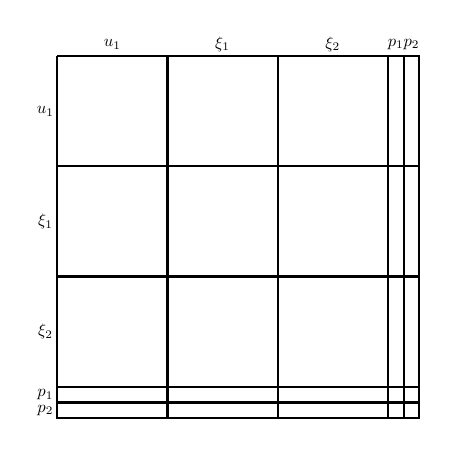
\begin{tikzpicture}[yscale=-1] 

\pgfmathsetmacro{\nt}{7};% time points
\pgfmathsetmacro{\nu}{1}; % controls
\pgfmathsetmacro{\nx}{2}; % states
\pgfmathsetmacro{\np}{2}; % parameters
\pgfmathsetmacro{\nc}{\nu + \nx}; % total continuous

%% control labels
\foreach \k in {1,...,\nu}{
	\pgfmathsetmacro{\x}{0.2*\nt*\k - 0.2/2*(\nt-1)};
	\node () at (\x,-0.05) {\scalebox{0.6}{$u_{\k}$}};
    \node () at (-0.05,\x) {\scalebox{0.6}{$u_{\k}$}};
}

%% state labels
\foreach \k in {1,...,\nx}{
	\pgfmathsetmacro{\x}{0.2*\nt*\k + 0.2*\nu*\nt - 0.2/2*(\nt-1)};
	\node () at (\x,-0.05) {\scalebox{0.6}{$\xi_{\k}$}};
    \node () at (-0.05,\x) {\scalebox{0.6}{$\xi_{\k}$}};
}

%% parameter labels
\foreach \k in {1,...,\np}{
	\pgfmathsetmacro{\x}{0.2*\k + 0.2*\nu*\nt + 0.2*\nx*\nt};
	\node () at (\x,-0.05) {\scalebox{0.6}{$p_{\k}$}};
    \node () at (-0.05,\x) {\scalebox{0.6}{$p_{\k}$}};
}


%% controls
\foreach \k in {1,...,\nu}{
	\foreach \j in {1,...,\nu}{
		\foreach \i in {1,...,\nt}{ 
        	\pgfmathsetmacro{\kk}{\k-1};
            \pgfmathsetmacro{\jj}{\j-1};
        	\pgfmathsetmacro{\x}{0.2*\i + 0.2*\kk*\nt};
            \pgfmathsetmacro{\y}{0.2*\i + 0.2*\jj*\nt};
        	\node () at (\x,\y) {\mysparsesymbol};
} 
    \pgfmathsetmacro{\kk}{\k-1};
    \pgfmathsetmacro{\jj}{\j-1};
    \pgfmathsetmacro{\x}{0.2*\kk*\nt + 0.1};
    \pgfmathsetmacro{\y}{0.2*\jj*\nt + 0.1};
	\draw[\mysparseboxcolor,thick](\x,\y) -- (\x+0.2*\nt,\y) -- (\x+0.2*\nt,\y+0.2*\nt) -- (\x,\y+0.2*\nt) -- (\x,\y);
} }

%% states
\foreach \k in {1,...,\nx}{
	\foreach \j in {1,...,\nx}{
		\foreach \i in {1,...,\nt}{ 
        	\pgfmathsetmacro{\kk}{\k-1};
            \pgfmathsetmacro{\jj}{\j-1};
        	\node () at (0.2*\i + 0.2*\kk*\nt + 0.2*\nu*\nt, 0.2*\i + 0.2*\jj*\nt + 0.2*\nu*\nt) {\mysparsesymbol};
} 
    \pgfmathsetmacro{\kk}{\k-1};
    \pgfmathsetmacro{\jj}{\j-1};
    \pgfmathsetmacro{\x}{0.2*\kk*\nt + 0.2*(\nu)*\nt + 0.1};
    \pgfmathsetmacro{\y}{0.2*\jj*\nt + 0.2*(\nu)*\nt + 0.1};
	\draw[\mysparseboxcolor,thick](\x,\y) -- (\x+0.2*\nt,\y) -- (\x+0.2*\nt,\y+0.2*\nt) -- (\x,\y+0.2*\nt) -- (\x,\y);
} }

%% parameters
\foreach \k in {1,...,\np}{
	\foreach \j in {1,...,\np}{
      \pgfmathsetmacro{\kk}{\k-1};
      \pgfmathsetmacro{\jj}{\j-1};
      \node ( ) at (0.2*\j + 0.2*\nx*\nt + 0.2*\nu*\nt, 0.2*\k + 0.2*\nx*\nt + 0.2*\nu*\nt) {\mysparsesymbol};
      \pgfmathsetmacro{\x}{0.2*\kk + 0.2*(\nu)*\nt + 0.2*\nx*\nt + 0.1};
      \pgfmathsetmacro{\y}{0.2*\jj + 0.2*(\nu)*\nt + 0.2*\nx*\nt + 0.1};
      \draw[\mysparseboxcolor,thick](\x,\y) -- (\x+0.2,\y) -- (\x+0.2,\y+0.2) -- (\x,\y+0.2) -- (\x,\y);
} }

%% states and controls
\foreach \k in {1,...,\nu}{
	\foreach \j in {1,...,\nx}{
		\foreach \i in {1,...,\nt}{ 
        	\pgfmathsetmacro{\kk}{\k-1};
            \pgfmathsetmacro{\jj}{\j-1};
        	\node () at ( 0.2*\i + 0.2*\kk*\nt , 0.2*\i + 0.2*\jj*\nt + 0.2*\nu*\nt) {\mysparsesymbol};
        	\node () at ( 0.2*\i + 0.2*\jj*\nt + 0.2*\nu*\nt, 0.2*\i + 0.2*\kk*\nt) {\mysparsesymbol};
} 
    \pgfmathsetmacro{\kk}{\k-1};
    \pgfmathsetmacro{\jj}{\j-1};
    \pgfmathsetmacro{\x}{0.2*\kk*\nt + 0.1};
    \pgfmathsetmacro{\y}{0.2*\jj*\nt + 0.2*(\nu)*\nt + 0.1};
	\draw[\mysparseboxcolor,thick](\x,\y) -- (\x+0.2*\nt,\y) -- (\x+0.2*\nt,\y+0.2*\nt) -- (\x,\y+0.2*\nt) -- (\x,\y);
    \draw[\mysparseboxcolor,thick](\y,\x) -- (\y+0.2*\nt,\x) -- (\y+0.2*\nt,\x+0.2*\nt) -- (\y,\x+0.2*\nt) -- (\y,\x);
} }

%% states and parameters
\foreach \k in {1,...,\np}{
	\foreach \j in {1,...,\nx}{
		\foreach \i in {1,...,\nt}{ 
        	\pgfmathsetmacro{\kk}{\k-1};
            \pgfmathsetmacro{\jj}{\j-1};
        	\node () at ( 0.2*\k + 0.2*\nx*\nt + 0.2*\nu*\nt, 0.2*\i + 0.2*\jj*\nt + 0.2*\nu*\nt ) {\mysparsesymbol};
            \node () at ( 0.2*\i + 0.2*\jj*\nt + 0.2*\nu*\nt, 0.2*\k + 0.2*\nx*\nt + 0.2*\nu*\nt ) {\mysparsesymbol};
} 
    \pgfmathsetmacro{\kk}{\k-1};
    \pgfmathsetmacro{\jj}{\j-1};
    \pgfmathsetmacro{\x}{0.2*\kk + 0.2*\nx*\nt + 0.2*\nu*\nt + 0.1};
    \pgfmathsetmacro{\y}{0.2*\jj*\nt + 0.2*\nu*\nt + 0.1};
	\draw[\mysparseboxcolor,thick](\x,\y) -- (\x+0.2,\y) -- (\x+0.2,\y+0.2*\nt) -- (\x,\y+0.2*\nt) -- (\x,\y);
    \draw[\mysparseboxcolor,thick](\y,\x) -- (\y+0.2*\nt,\x) -- (\y+0.2*\nt,\x+0.2) -- (\y,\x+0.2) -- (\y,\x);

} }

%% controls and parameters
\foreach \k in {1,...,\np}{
	\foreach \j in {1,...,\nu}{
		\foreach \i in {1,...,\nt}{ 
        	\pgfmathsetmacro{\kk}{\k-1};
            \pgfmathsetmacro{\jj}{\j-1};
        	\node () at ( 0.2*\k + 0.2*\nx*\nt + 0.2*\nu*\nt, 0.2*\i + 0.2*\jj*\nt ) {\mysparsesymbol};
            \node () at ( 0.2*\i + 0.2*\jj*\nt , 0.2*\k + 0.2*\nx*\nt + 0.2*\nu*\nt ) {\mysparsesymbol};
} 
    \pgfmathsetmacro{\kk}{\k-1};
    \pgfmathsetmacro{\jj}{\j-1};
    \pgfmathsetmacro{\x}{0.2*\kk + 0.2*\nx*\nt + 0.2*\nu*\nt + 0.1};
    \pgfmathsetmacro{\y}{0.2*\jj*\nt + 0.1};
	\draw[\mysparseboxcolor,thick](\x,\y) -- (\x+0.2,\y) -- (\x+0.2,\y+0.2*\nt) -- (\x,\y+0.2*\nt) -- (\x,\y);
    \draw[\mysparseboxcolor,thick](\y,\x) -- (\y+0.2*\nt,\x) -- (\y+0.2*\nt,\x+0.2) -- (\y,\x+0.2) -- (\y,\x);
} }

%% initial states
\foreach \k in {1,...,\nx}{
	\foreach \j in {1,...,\nc}{
		\foreach \i in {1,...,\nt}{ 
        	\pgfmathsetmacro{\kk}{\k-1};
            \pgfmathsetmacro{\jj}{\j-1};
        	\node () at (0.2 + 0.2*\kk*\nt + 0.2*\nu*\nt, 0.2*\i + 0.2*\jj*\nt ) {\mysparsesymbol};
            \node () at ( 0.2*\i + 0.2*\jj*\nt , 0.2 + 0.2*\kk*\nt + 0.2*\nu*\nt ) {\mysparsesymbol};
} } 
	\foreach \j in {1,...,\np}{
		\pgfmathsetmacro{\kk}{\k-1};
        \pgfmathsetmacro{\jj}{\j-1};
        \node () at ( 0.2*\k + 0.2*\nx*\nt + 0.2*\nu*\nt, 0.2 + 0.2*\jj*\nt + 0.2*\nu*\nt ) {\mysparsesymbol};
        \node () at ( 0.2 + 0.2*\jj*\nt + 0.2*\nu*\nt , 0.2*\k + 0.2*\nx*\nt + 0.2*\nu*\nt ) {\mysparsesymbol};
	}
}

%% final states
\foreach \k in {1,...,\nx}{
	\foreach \j in {1,...,\nc}{
		\foreach \i in {1,...,\nt}{ 
        	\pgfmathsetmacro{\kk}{\k-1};
            \pgfmathsetmacro{\jj}{\j-1};
        	\node () at (0.2*\nt + 0.2*\kk*\nt + 0.2*\nu*\nt, 0.2*\i + 0.2*\jj*\nt ) {\mysparsesymbol};
            \node () at ( 0.2*\i + 0.2*\jj*\nt , 0.2*\nt + 0.2*\kk*\nt + 0.2*\nu*\nt ) {\mysparsesymbol};
} } 
	\foreach \j in {1,...,\np}{
		\pgfmathsetmacro{\kk}{\k-1};
        \pgfmathsetmacro{\jj}{\j-1};
        \node () at ( 0.2*\k + 0.2*\nx*\nt + 0.2*\nu*\nt, 0.2*\nt + 0.2*\jj*\nt + 0.2*\nu*\nt ) {\mysparsesymbol};
        \node () at ( 0.2*\nt + 0.2*\jj*\nt + 0.2*\nu*\nt , 0.2*\k + 0.2*\nx*\nt + 0.2*\nu*\nt ) {\mysparsesymbol};
	}
}


























% %% states and controls
% \foreach \k in {0,...,2}{
% 	\foreach \j in {0,...,2}{
% 		\foreach \i in {1,...,5}{ 
%         	\node () at (0.2*\i + \k,0.2*\i + \j) {\mysparsesymbol};
% } } }

% %% parameters - right
% \foreach \k in {0,...,1}{
% 	\foreach \j in {0,...,2}{
% 		\foreach \i in {1,...,5}{
%         	\node ( ) at (0.2*\k + 3.2, 0.2*\i + \j) {\mysparsesymbol};
% } } }

% %% parameters - bottom
% \foreach \k in {0,...,1}{
% 	\foreach \j in {0,...,2}{
% 		\foreach \i in {1,...,5}{
%         	\node ( ) at (0.2*\i + \j, 0.2*\k + 3.2) {\mysparsesymbol};
% } } }

% %% parameters - corner
% \foreach \k in {0,...,1}{
% 	\foreach \j in {0,...,1}{
%         	\node ( ) at (0.2*\j + 3.2, 0.2*\k + 3.2) {\mysparsesymbol};
% } }

% %% initial states - bottom
% \foreach \k in {0,...,1}{
% 	\foreach \j in {0,...,2}{
% 		\foreach \i in {1,...,5}{
%         	\node ( ) at (0.2*\i + \j, \k + 1.2) {\mysparsesymbol};
% } } }

% %% final states - bottom
% \foreach \k in {0,...,1}{
% 	\foreach \j in {0,...,2}{
% 		\foreach \i in {1,...,5}{
%         	\node ( ) at (0.2*\i + \j, \k + 2.0) {\mysparsesymbol};
% } } }

% %% initial states - right
% \foreach \k in {0,...,1}{
% 	\foreach \j in {0,...,2}{
% 		\foreach \i in {1,...,5}{
%         	\node ( ) at (\k + 1.2, 0.2*\i + \j) {\mysparsesymbol};
% } } }

% %% final states - right
% \foreach \k in {0,...,1}{
% 	\foreach \j in {0,...,2}{
% 		\foreach \i in {1,...,5}{
%         	\node ( ) at (\k + 2.0, 0.2*\i + \j) {\mysparsesymbol};
% } } }


% %% draw boxes - states and controls
% \foreach \k in {0,...,2}{
% 	\foreach \j in {0,...,2}{
%     	\pgfmathsetmacro{\x}{\k + 0.1};
%     	\pgfmathsetmacro{\y}{\j + 0.1};
%         \draw[blue!70] (\x,\y) -- (\x+1,\y) -- (\x+1,\y+1) -- (\x,\y+1) -- (\x,\y);
% } }

% %% draw boxes - parameters - right
% \foreach \k in {0,...,1}{
% 	\foreach \j in {0,...,2}{
%     	\pgfmathsetmacro{\x}{0.2*\k + 0.1 + 3};
%     	\pgfmathsetmacro{\y}{\j + 0.1};
%         \draw[blue] (\x,\y) -- (\x+0.2,\y) -- (\x+0.2,\y+1) -- (\x,\y+1) -- (\x,\y);
% } }

% %% draw boxes - parameters - bottom
% \foreach \k in {0,...,2}{
% 	\foreach \j in {0,...,1}{
%     	\pgfmathsetmacro{\x}{\k + 0.1};
%     	\pgfmathsetmacro{\y}{0.2*\j + 0.1 + 3};
%         \draw[blue] (\x,\y) -- (\x+1,\y) -- (\x+1,\y+0.2) -- (\x,\y+0.2) -- (\x,\y);
% } }

% %% draw boxes - parameters - bottom
% \foreach \k in {0,...,1}{
% 	\foreach \j in {0,...,1}{
%     	\pgfmathsetmacro{\x}{0.2*\k + 0.1 + 3};
%     	\pgfmathsetmacro{\y}{0.2*\j + 0.1 + 3};
%         \draw[blue] (\x,\y) -- (\x+0.2,\y) -- (\x+0.2,\y+0.2) -- (\x,\y+0.2) -- (\x,\y);
% } }


%% states
\foreach \k in {1,...,\nx}{
	\foreach \j in {1,...,\nx}{
		\foreach \i in {1,...,\nt}{ 
        	\pgfmathsetmacro{\kk}{\k-1};
            \pgfmathsetmacro{\jj}{\j-1};
        	\node () at (0.2*\i + 0.2*\kk*\nt + 0.2*\nu*\nt, 0.2*\i + 0.2*\jj*\nt + 0.2*\nu*\nt) {\mytemp};
} } }
\end{tikzpicture}
}
\vspace{-5mm}
\caption{$\bm{L}_{22}$ terms.}
\end{subfigure}

\begin{subfigure}[b]{0.45\textwidth}
\tikzsetnextfilename{Hpp}

\centering
\resizebox{1\textwidth}{!}{
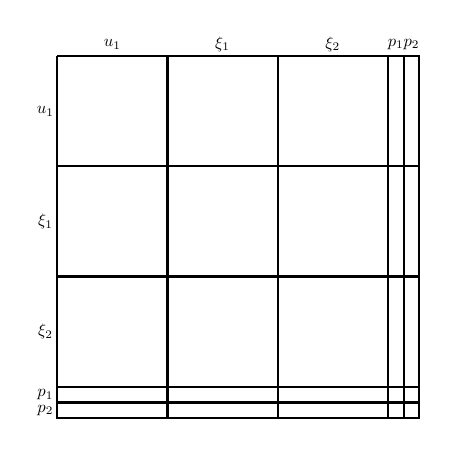
\begin{tikzpicture}[yscale=-1] 

\pgfmathsetmacro{\nt}{7};% time points
\pgfmathsetmacro{\nu}{1}; % controls
\pgfmathsetmacro{\nx}{2}; % states
\pgfmathsetmacro{\np}{2}; % parameters
\pgfmathsetmacro{\nc}{\nu + \nx}; % total continuous

%% control labels
\foreach \k in {1,...,\nu}{
	\pgfmathsetmacro{\x}{0.2*\nt*\k - 0.2/2*(\nt-1)};
	\node () at (\x,-0.05) {\scalebox{0.6}{$u_{\k}$}};
    \node () at (-0.05,\x) {\scalebox{0.6}{$u_{\k}$}};
}

%% state labels
\foreach \k in {1,...,\nx}{
	\pgfmathsetmacro{\x}{0.2*\nt*\k + 0.2*\nu*\nt - 0.2/2*(\nt-1)};
	\node () at (\x,-0.05) {\scalebox{0.6}{$\xi_{\k}$}};
    \node () at (-0.05,\x) {\scalebox{0.6}{$\xi_{\k}$}};
}

%% parameter labels
\foreach \k in {1,...,\np}{
	\pgfmathsetmacro{\x}{0.2*\k + 0.2*\nu*\nt + 0.2*\nx*\nt};
	\node () at (\x,-0.05) {\scalebox{0.6}{$p_{\k}$}};
    \node () at (-0.05,\x) {\scalebox{0.6}{$p_{\k}$}};
}


%% controls
\foreach \k in {1,...,\nu}{
	\foreach \j in {1,...,\nu}{
		\foreach \i in {1,...,\nt}{ 
        	\pgfmathsetmacro{\kk}{\k-1};
            \pgfmathsetmacro{\jj}{\j-1};
        	\pgfmathsetmacro{\x}{0.2*\i + 0.2*\kk*\nt};
            \pgfmathsetmacro{\y}{0.2*\i + 0.2*\jj*\nt};
        	\node () at (\x,\y) {\mysparsesymbol};
} 
    \pgfmathsetmacro{\kk}{\k-1};
    \pgfmathsetmacro{\jj}{\j-1};
    \pgfmathsetmacro{\x}{0.2*\kk*\nt + 0.1};
    \pgfmathsetmacro{\y}{0.2*\jj*\nt + 0.1};
	\draw[\mysparseboxcolor,thick](\x,\y) -- (\x+0.2*\nt,\y) -- (\x+0.2*\nt,\y+0.2*\nt) -- (\x,\y+0.2*\nt) -- (\x,\y);
} }

%% states
\foreach \k in {1,...,\nx}{
	\foreach \j in {1,...,\nx}{
		\foreach \i in {1,...,\nt}{ 
        	\pgfmathsetmacro{\kk}{\k-1};
            \pgfmathsetmacro{\jj}{\j-1};
        	\node () at (0.2*\i + 0.2*\kk*\nt + 0.2*\nu*\nt, 0.2*\i + 0.2*\jj*\nt + 0.2*\nu*\nt) {\mysparsesymbol};
} 
    \pgfmathsetmacro{\kk}{\k-1};
    \pgfmathsetmacro{\jj}{\j-1};
    \pgfmathsetmacro{\x}{0.2*\kk*\nt + 0.2*(\nu)*\nt + 0.1};
    \pgfmathsetmacro{\y}{0.2*\jj*\nt + 0.2*(\nu)*\nt + 0.1};
	\draw[\mysparseboxcolor,thick](\x,\y) -- (\x+0.2*\nt,\y) -- (\x+0.2*\nt,\y+0.2*\nt) -- (\x,\y+0.2*\nt) -- (\x,\y);
} }

%% parameters
\foreach \k in {1,...,\np}{
	\foreach \j in {1,...,\np}{
      \pgfmathsetmacro{\kk}{\k-1};
      \pgfmathsetmacro{\jj}{\j-1};
      \node ( ) at (0.2*\j + 0.2*\nx*\nt + 0.2*\nu*\nt, 0.2*\k + 0.2*\nx*\nt + 0.2*\nu*\nt) {\mysparsesymbol};
      \pgfmathsetmacro{\x}{0.2*\kk + 0.2*(\nu)*\nt + 0.2*\nx*\nt + 0.1};
      \pgfmathsetmacro{\y}{0.2*\jj + 0.2*(\nu)*\nt + 0.2*\nx*\nt + 0.1};
      \draw[\mysparseboxcolor,thick](\x,\y) -- (\x+0.2,\y) -- (\x+0.2,\y+0.2) -- (\x,\y+0.2) -- (\x,\y);
} }

%% states and controls
\foreach \k in {1,...,\nu}{
	\foreach \j in {1,...,\nx}{
		\foreach \i in {1,...,\nt}{ 
        	\pgfmathsetmacro{\kk}{\k-1};
            \pgfmathsetmacro{\jj}{\j-1};
        	\node () at ( 0.2*\i + 0.2*\kk*\nt , 0.2*\i + 0.2*\jj*\nt + 0.2*\nu*\nt) {\mysparsesymbol};
        	\node () at ( 0.2*\i + 0.2*\jj*\nt + 0.2*\nu*\nt, 0.2*\i + 0.2*\kk*\nt) {\mysparsesymbol};
} 
    \pgfmathsetmacro{\kk}{\k-1};
    \pgfmathsetmacro{\jj}{\j-1};
    \pgfmathsetmacro{\x}{0.2*\kk*\nt + 0.1};
    \pgfmathsetmacro{\y}{0.2*\jj*\nt + 0.2*(\nu)*\nt + 0.1};
	\draw[\mysparseboxcolor,thick](\x,\y) -- (\x+0.2*\nt,\y) -- (\x+0.2*\nt,\y+0.2*\nt) -- (\x,\y+0.2*\nt) -- (\x,\y);
    \draw[\mysparseboxcolor,thick](\y,\x) -- (\y+0.2*\nt,\x) -- (\y+0.2*\nt,\x+0.2*\nt) -- (\y,\x+0.2*\nt) -- (\y,\x);
} }

%% states and parameters
\foreach \k in {1,...,\np}{
	\foreach \j in {1,...,\nx}{
		\foreach \i in {1,...,\nt}{ 
        	\pgfmathsetmacro{\kk}{\k-1};
            \pgfmathsetmacro{\jj}{\j-1};
        	\node () at ( 0.2*\k + 0.2*\nx*\nt + 0.2*\nu*\nt, 0.2*\i + 0.2*\jj*\nt + 0.2*\nu*\nt ) {\mysparsesymbol};
            \node () at ( 0.2*\i + 0.2*\jj*\nt + 0.2*\nu*\nt, 0.2*\k + 0.2*\nx*\nt + 0.2*\nu*\nt ) {\mysparsesymbol};
} 
    \pgfmathsetmacro{\kk}{\k-1};
    \pgfmathsetmacro{\jj}{\j-1};
    \pgfmathsetmacro{\x}{0.2*\kk + 0.2*\nx*\nt + 0.2*\nu*\nt + 0.1};
    \pgfmathsetmacro{\y}{0.2*\jj*\nt + 0.2*\nu*\nt + 0.1};
	\draw[\mysparseboxcolor,thick](\x,\y) -- (\x+0.2,\y) -- (\x+0.2,\y+0.2*\nt) -- (\x,\y+0.2*\nt) -- (\x,\y);
    \draw[\mysparseboxcolor,thick](\y,\x) -- (\y+0.2*\nt,\x) -- (\y+0.2*\nt,\x+0.2) -- (\y,\x+0.2) -- (\y,\x);

} }

%% controls and parameters
\foreach \k in {1,...,\np}{
	\foreach \j in {1,...,\nu}{
		\foreach \i in {1,...,\nt}{ 
        	\pgfmathsetmacro{\kk}{\k-1};
            \pgfmathsetmacro{\jj}{\j-1};
        	\node () at ( 0.2*\k + 0.2*\nx*\nt + 0.2*\nu*\nt, 0.2*\i + 0.2*\jj*\nt ) {\mysparsesymbol};
            \node () at ( 0.2*\i + 0.2*\jj*\nt , 0.2*\k + 0.2*\nx*\nt + 0.2*\nu*\nt ) {\mysparsesymbol};
} 
    \pgfmathsetmacro{\kk}{\k-1};
    \pgfmathsetmacro{\jj}{\j-1};
    \pgfmathsetmacro{\x}{0.2*\kk + 0.2*\nx*\nt + 0.2*\nu*\nt + 0.1};
    \pgfmathsetmacro{\y}{0.2*\jj*\nt + 0.1};
	\draw[\mysparseboxcolor,thick](\x,\y) -- (\x+0.2,\y) -- (\x+0.2,\y+0.2*\nt) -- (\x,\y+0.2*\nt) -- (\x,\y);
    \draw[\mysparseboxcolor,thick](\y,\x) -- (\y+0.2*\nt,\x) -- (\y+0.2*\nt,\x+0.2) -- (\y,\x+0.2) -- (\y,\x);
} }

%% initial states
\foreach \k in {1,...,\nx}{
	\foreach \j in {1,...,\nc}{
		\foreach \i in {1,...,\nt}{ 
        	\pgfmathsetmacro{\kk}{\k-1};
            \pgfmathsetmacro{\jj}{\j-1};
        	\node () at (0.2 + 0.2*\kk*\nt + 0.2*\nu*\nt, 0.2*\i + 0.2*\jj*\nt ) {\mysparsesymbol};
            \node () at ( 0.2*\i + 0.2*\jj*\nt , 0.2 + 0.2*\kk*\nt + 0.2*\nu*\nt ) {\mysparsesymbol};
} } 
	\foreach \j in {1,...,\np}{
		\pgfmathsetmacro{\kk}{\k-1};
        \pgfmathsetmacro{\jj}{\j-1};
        \node () at ( 0.2*\k + 0.2*\nx*\nt + 0.2*\nu*\nt, 0.2 + 0.2*\jj*\nt + 0.2*\nu*\nt ) {\mysparsesymbol};
        \node () at ( 0.2 + 0.2*\jj*\nt + 0.2*\nu*\nt , 0.2*\k + 0.2*\nx*\nt + 0.2*\nu*\nt ) {\mysparsesymbol};
	}
}

%% final states
\foreach \k in {1,...,\nx}{
	\foreach \j in {1,...,\nc}{
		\foreach \i in {1,...,\nt}{ 
        	\pgfmathsetmacro{\kk}{\k-1};
            \pgfmathsetmacro{\jj}{\j-1};
        	\node () at (0.2*\nt + 0.2*\kk*\nt + 0.2*\nu*\nt, 0.2*\i + 0.2*\jj*\nt ) {\mysparsesymbol};
            \node () at ( 0.2*\i + 0.2*\jj*\nt , 0.2*\nt + 0.2*\kk*\nt + 0.2*\nu*\nt ) {\mysparsesymbol};
} } 
	\foreach \j in {1,...,\np}{
		\pgfmathsetmacro{\kk}{\k-1};
        \pgfmathsetmacro{\jj}{\j-1};
        \node () at ( 0.2*\k + 0.2*\nx*\nt + 0.2*\nu*\nt, 0.2*\nt + 0.2*\jj*\nt + 0.2*\nu*\nt ) {\mysparsesymbol};
        \node () at ( 0.2*\nt + 0.2*\jj*\nt + 0.2*\nu*\nt , 0.2*\k + 0.2*\nx*\nt + 0.2*\nu*\nt ) {\mysparsesymbol};
	}
}


























% %% states and controls
% \foreach \k in {0,...,2}{
% 	\foreach \j in {0,...,2}{
% 		\foreach \i in {1,...,5}{ 
%         	\node () at (0.2*\i + \k,0.2*\i + \j) {\mysparsesymbol};
% } } }

% %% parameters - right
% \foreach \k in {0,...,1}{
% 	\foreach \j in {0,...,2}{
% 		\foreach \i in {1,...,5}{
%         	\node ( ) at (0.2*\k + 3.2, 0.2*\i + \j) {\mysparsesymbol};
% } } }

% %% parameters - bottom
% \foreach \k in {0,...,1}{
% 	\foreach \j in {0,...,2}{
% 		\foreach \i in {1,...,5}{
%         	\node ( ) at (0.2*\i + \j, 0.2*\k + 3.2) {\mysparsesymbol};
% } } }

% %% parameters - corner
% \foreach \k in {0,...,1}{
% 	\foreach \j in {0,...,1}{
%         	\node ( ) at (0.2*\j + 3.2, 0.2*\k + 3.2) {\mysparsesymbol};
% } }

% %% initial states - bottom
% \foreach \k in {0,...,1}{
% 	\foreach \j in {0,...,2}{
% 		\foreach \i in {1,...,5}{
%         	\node ( ) at (0.2*\i + \j, \k + 1.2) {\mysparsesymbol};
% } } }

% %% final states - bottom
% \foreach \k in {0,...,1}{
% 	\foreach \j in {0,...,2}{
% 		\foreach \i in {1,...,5}{
%         	\node ( ) at (0.2*\i + \j, \k + 2.0) {\mysparsesymbol};
% } } }

% %% initial states - right
% \foreach \k in {0,...,1}{
% 	\foreach \j in {0,...,2}{
% 		\foreach \i in {1,...,5}{
%         	\node ( ) at (\k + 1.2, 0.2*\i + \j) {\mysparsesymbol};
% } } }

% %% final states - right
% \foreach \k in {0,...,1}{
% 	\foreach \j in {0,...,2}{
% 		\foreach \i in {1,...,5}{
%         	\node ( ) at (\k + 2.0, 0.2*\i + \j) {\mysparsesymbol};
% } } }


% %% draw boxes - states and controls
% \foreach \k in {0,...,2}{
% 	\foreach \j in {0,...,2}{
%     	\pgfmathsetmacro{\x}{\k + 0.1};
%     	\pgfmathsetmacro{\y}{\j + 0.1};
%         \draw[blue!70] (\x,\y) -- (\x+1,\y) -- (\x+1,\y+1) -- (\x,\y+1) -- (\x,\y);
% } }

% %% draw boxes - parameters - right
% \foreach \k in {0,...,1}{
% 	\foreach \j in {0,...,2}{
%     	\pgfmathsetmacro{\x}{0.2*\k + 0.1 + 3};
%     	\pgfmathsetmacro{\y}{\j + 0.1};
%         \draw[blue] (\x,\y) -- (\x+0.2,\y) -- (\x+0.2,\y+1) -- (\x,\y+1) -- (\x,\y);
% } }

% %% draw boxes - parameters - bottom
% \foreach \k in {0,...,2}{
% 	\foreach \j in {0,...,1}{
%     	\pgfmathsetmacro{\x}{\k + 0.1};
%     	\pgfmathsetmacro{\y}{0.2*\j + 0.1 + 3};
%         \draw[blue] (\x,\y) -- (\x+1,\y) -- (\x+1,\y+0.2) -- (\x,\y+0.2) -- (\x,\y);
% } }

% %% draw boxes - parameters - bottom
% \foreach \k in {0,...,1}{
% 	\foreach \j in {0,...,1}{
%     	\pgfmathsetmacro{\x}{0.2*\k + 0.1 + 3};
%     	\pgfmathsetmacro{\y}{0.2*\j + 0.1 + 3};
%         \draw[blue] (\x,\y) -- (\x+0.2,\y) -- (\x+0.2,\y+0.2) -- (\x,\y+0.2) -- (\x,\y);
% } }


%% parameters
\foreach \k in {1,...,\np}{
	\foreach \j in {1,...,\np}{
      \pgfmathsetmacro{\kk}{\k-1};
      \pgfmathsetmacro{\jj}{\j-1};
      \node ( ) at (0.2*\j + 0.2*\nx*\nt + 0.2*\nu*\nt, 0.2*\k + 0.2*\nx*\nt + 0.2*\nu*\nt) {\mytemp};
} }
\end{tikzpicture}
}
\vspace{-5mm}
\caption{$\bm{L}_{33}$ terms.}
\end{subfigure}
%%%%%%%%%%%
\begin{subfigure}[b]{0.45\textwidth}
\tikzsetnextfilename{Hx0x0}

\centering
\resizebox{1\textwidth}{!}{
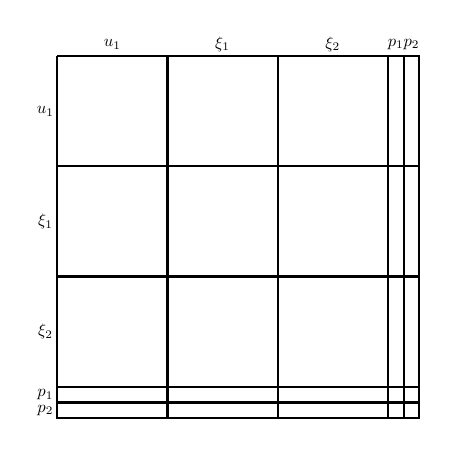
\begin{tikzpicture}[yscale=-1] 

\pgfmathsetmacro{\nt}{7};% time points
\pgfmathsetmacro{\nu}{1}; % controls
\pgfmathsetmacro{\nx}{2}; % states
\pgfmathsetmacro{\np}{2}; % parameters
\pgfmathsetmacro{\nc}{\nu + \nx}; % total continuous

%% control labels
\foreach \k in {1,...,\nu}{
	\pgfmathsetmacro{\x}{0.2*\nt*\k - 0.2/2*(\nt-1)};
	\node () at (\x,-0.05) {\scalebox{0.6}{$u_{\k}$}};
    \node () at (-0.05,\x) {\scalebox{0.6}{$u_{\k}$}};
}

%% state labels
\foreach \k in {1,...,\nx}{
	\pgfmathsetmacro{\x}{0.2*\nt*\k + 0.2*\nu*\nt - 0.2/2*(\nt-1)};
	\node () at (\x,-0.05) {\scalebox{0.6}{$\xi_{\k}$}};
    \node () at (-0.05,\x) {\scalebox{0.6}{$\xi_{\k}$}};
}

%% parameter labels
\foreach \k in {1,...,\np}{
	\pgfmathsetmacro{\x}{0.2*\k + 0.2*\nu*\nt + 0.2*\nx*\nt};
	\node () at (\x,-0.05) {\scalebox{0.6}{$p_{\k}$}};
    \node () at (-0.05,\x) {\scalebox{0.6}{$p_{\k}$}};
}


%% controls
\foreach \k in {1,...,\nu}{
	\foreach \j in {1,...,\nu}{
		\foreach \i in {1,...,\nt}{ 
        	\pgfmathsetmacro{\kk}{\k-1};
            \pgfmathsetmacro{\jj}{\j-1};
        	\pgfmathsetmacro{\x}{0.2*\i + 0.2*\kk*\nt};
            \pgfmathsetmacro{\y}{0.2*\i + 0.2*\jj*\nt};
        	\node () at (\x,\y) {\mysparsesymbol};
} 
    \pgfmathsetmacro{\kk}{\k-1};
    \pgfmathsetmacro{\jj}{\j-1};
    \pgfmathsetmacro{\x}{0.2*\kk*\nt + 0.1};
    \pgfmathsetmacro{\y}{0.2*\jj*\nt + 0.1};
	\draw[\mysparseboxcolor,thick](\x,\y) -- (\x+0.2*\nt,\y) -- (\x+0.2*\nt,\y+0.2*\nt) -- (\x,\y+0.2*\nt) -- (\x,\y);
} }

%% states
\foreach \k in {1,...,\nx}{
	\foreach \j in {1,...,\nx}{
		\foreach \i in {1,...,\nt}{ 
        	\pgfmathsetmacro{\kk}{\k-1};
            \pgfmathsetmacro{\jj}{\j-1};
        	\node () at (0.2*\i + 0.2*\kk*\nt + 0.2*\nu*\nt, 0.2*\i + 0.2*\jj*\nt + 0.2*\nu*\nt) {\mysparsesymbol};
} 
    \pgfmathsetmacro{\kk}{\k-1};
    \pgfmathsetmacro{\jj}{\j-1};
    \pgfmathsetmacro{\x}{0.2*\kk*\nt + 0.2*(\nu)*\nt + 0.1};
    \pgfmathsetmacro{\y}{0.2*\jj*\nt + 0.2*(\nu)*\nt + 0.1};
	\draw[\mysparseboxcolor,thick](\x,\y) -- (\x+0.2*\nt,\y) -- (\x+0.2*\nt,\y+0.2*\nt) -- (\x,\y+0.2*\nt) -- (\x,\y);
} }

%% parameters
\foreach \k in {1,...,\np}{
	\foreach \j in {1,...,\np}{
      \pgfmathsetmacro{\kk}{\k-1};
      \pgfmathsetmacro{\jj}{\j-1};
      \node ( ) at (0.2*\j + 0.2*\nx*\nt + 0.2*\nu*\nt, 0.2*\k + 0.2*\nx*\nt + 0.2*\nu*\nt) {\mysparsesymbol};
      \pgfmathsetmacro{\x}{0.2*\kk + 0.2*(\nu)*\nt + 0.2*\nx*\nt + 0.1};
      \pgfmathsetmacro{\y}{0.2*\jj + 0.2*(\nu)*\nt + 0.2*\nx*\nt + 0.1};
      \draw[\mysparseboxcolor,thick](\x,\y) -- (\x+0.2,\y) -- (\x+0.2,\y+0.2) -- (\x,\y+0.2) -- (\x,\y);
} }

%% states and controls
\foreach \k in {1,...,\nu}{
	\foreach \j in {1,...,\nx}{
		\foreach \i in {1,...,\nt}{ 
        	\pgfmathsetmacro{\kk}{\k-1};
            \pgfmathsetmacro{\jj}{\j-1};
        	\node () at ( 0.2*\i + 0.2*\kk*\nt , 0.2*\i + 0.2*\jj*\nt + 0.2*\nu*\nt) {\mysparsesymbol};
        	\node () at ( 0.2*\i + 0.2*\jj*\nt + 0.2*\nu*\nt, 0.2*\i + 0.2*\kk*\nt) {\mysparsesymbol};
} 
    \pgfmathsetmacro{\kk}{\k-1};
    \pgfmathsetmacro{\jj}{\j-1};
    \pgfmathsetmacro{\x}{0.2*\kk*\nt + 0.1};
    \pgfmathsetmacro{\y}{0.2*\jj*\nt + 0.2*(\nu)*\nt + 0.1};
	\draw[\mysparseboxcolor,thick](\x,\y) -- (\x+0.2*\nt,\y) -- (\x+0.2*\nt,\y+0.2*\nt) -- (\x,\y+0.2*\nt) -- (\x,\y);
    \draw[\mysparseboxcolor,thick](\y,\x) -- (\y+0.2*\nt,\x) -- (\y+0.2*\nt,\x+0.2*\nt) -- (\y,\x+0.2*\nt) -- (\y,\x);
} }

%% states and parameters
\foreach \k in {1,...,\np}{
	\foreach \j in {1,...,\nx}{
		\foreach \i in {1,...,\nt}{ 
        	\pgfmathsetmacro{\kk}{\k-1};
            \pgfmathsetmacro{\jj}{\j-1};
        	\node () at ( 0.2*\k + 0.2*\nx*\nt + 0.2*\nu*\nt, 0.2*\i + 0.2*\jj*\nt + 0.2*\nu*\nt ) {\mysparsesymbol};
            \node () at ( 0.2*\i + 0.2*\jj*\nt + 0.2*\nu*\nt, 0.2*\k + 0.2*\nx*\nt + 0.2*\nu*\nt ) {\mysparsesymbol};
} 
    \pgfmathsetmacro{\kk}{\k-1};
    \pgfmathsetmacro{\jj}{\j-1};
    \pgfmathsetmacro{\x}{0.2*\kk + 0.2*\nx*\nt + 0.2*\nu*\nt + 0.1};
    \pgfmathsetmacro{\y}{0.2*\jj*\nt + 0.2*\nu*\nt + 0.1};
	\draw[\mysparseboxcolor,thick](\x,\y) -- (\x+0.2,\y) -- (\x+0.2,\y+0.2*\nt) -- (\x,\y+0.2*\nt) -- (\x,\y);
    \draw[\mysparseboxcolor,thick](\y,\x) -- (\y+0.2*\nt,\x) -- (\y+0.2*\nt,\x+0.2) -- (\y,\x+0.2) -- (\y,\x);

} }

%% controls and parameters
\foreach \k in {1,...,\np}{
	\foreach \j in {1,...,\nu}{
		\foreach \i in {1,...,\nt}{ 
        	\pgfmathsetmacro{\kk}{\k-1};
            \pgfmathsetmacro{\jj}{\j-1};
        	\node () at ( 0.2*\k + 0.2*\nx*\nt + 0.2*\nu*\nt, 0.2*\i + 0.2*\jj*\nt ) {\mysparsesymbol};
            \node () at ( 0.2*\i + 0.2*\jj*\nt , 0.2*\k + 0.2*\nx*\nt + 0.2*\nu*\nt ) {\mysparsesymbol};
} 
    \pgfmathsetmacro{\kk}{\k-1};
    \pgfmathsetmacro{\jj}{\j-1};
    \pgfmathsetmacro{\x}{0.2*\kk + 0.2*\nx*\nt + 0.2*\nu*\nt + 0.1};
    \pgfmathsetmacro{\y}{0.2*\jj*\nt + 0.1};
	\draw[\mysparseboxcolor,thick](\x,\y) -- (\x+0.2,\y) -- (\x+0.2,\y+0.2*\nt) -- (\x,\y+0.2*\nt) -- (\x,\y);
    \draw[\mysparseboxcolor,thick](\y,\x) -- (\y+0.2*\nt,\x) -- (\y+0.2*\nt,\x+0.2) -- (\y,\x+0.2) -- (\y,\x);
} }

%% initial states
\foreach \k in {1,...,\nx}{
	\foreach \j in {1,...,\nc}{
		\foreach \i in {1,...,\nt}{ 
        	\pgfmathsetmacro{\kk}{\k-1};
            \pgfmathsetmacro{\jj}{\j-1};
        	\node () at (0.2 + 0.2*\kk*\nt + 0.2*\nu*\nt, 0.2*\i + 0.2*\jj*\nt ) {\mysparsesymbol};
            \node () at ( 0.2*\i + 0.2*\jj*\nt , 0.2 + 0.2*\kk*\nt + 0.2*\nu*\nt ) {\mysparsesymbol};
} } 
	\foreach \j in {1,...,\np}{
		\pgfmathsetmacro{\kk}{\k-1};
        \pgfmathsetmacro{\jj}{\j-1};
        \node () at ( 0.2*\k + 0.2*\nx*\nt + 0.2*\nu*\nt, 0.2 + 0.2*\jj*\nt + 0.2*\nu*\nt ) {\mysparsesymbol};
        \node () at ( 0.2 + 0.2*\jj*\nt + 0.2*\nu*\nt , 0.2*\k + 0.2*\nx*\nt + 0.2*\nu*\nt ) {\mysparsesymbol};
	}
}

%% final states
\foreach \k in {1,...,\nx}{
	\foreach \j in {1,...,\nc}{
		\foreach \i in {1,...,\nt}{ 
        	\pgfmathsetmacro{\kk}{\k-1};
            \pgfmathsetmacro{\jj}{\j-1};
        	\node () at (0.2*\nt + 0.2*\kk*\nt + 0.2*\nu*\nt, 0.2*\i + 0.2*\jj*\nt ) {\mysparsesymbol};
            \node () at ( 0.2*\i + 0.2*\jj*\nt , 0.2*\nt + 0.2*\kk*\nt + 0.2*\nu*\nt ) {\mysparsesymbol};
} } 
	\foreach \j in {1,...,\np}{
		\pgfmathsetmacro{\kk}{\k-1};
        \pgfmathsetmacro{\jj}{\j-1};
        \node () at ( 0.2*\k + 0.2*\nx*\nt + 0.2*\nu*\nt, 0.2*\nt + 0.2*\jj*\nt + 0.2*\nu*\nt ) {\mysparsesymbol};
        \node () at ( 0.2*\nt + 0.2*\jj*\nt + 0.2*\nu*\nt , 0.2*\k + 0.2*\nx*\nt + 0.2*\nu*\nt ) {\mysparsesymbol};
	}
}


























% %% states and controls
% \foreach \k in {0,...,2}{
% 	\foreach \j in {0,...,2}{
% 		\foreach \i in {1,...,5}{ 
%         	\node () at (0.2*\i + \k,0.2*\i + \j) {\mysparsesymbol};
% } } }

% %% parameters - right
% \foreach \k in {0,...,1}{
% 	\foreach \j in {0,...,2}{
% 		\foreach \i in {1,...,5}{
%         	\node ( ) at (0.2*\k + 3.2, 0.2*\i + \j) {\mysparsesymbol};
% } } }

% %% parameters - bottom
% \foreach \k in {0,...,1}{
% 	\foreach \j in {0,...,2}{
% 		\foreach \i in {1,...,5}{
%         	\node ( ) at (0.2*\i + \j, 0.2*\k + 3.2) {\mysparsesymbol};
% } } }

% %% parameters - corner
% \foreach \k in {0,...,1}{
% 	\foreach \j in {0,...,1}{
%         	\node ( ) at (0.2*\j + 3.2, 0.2*\k + 3.2) {\mysparsesymbol};
% } }

% %% initial states - bottom
% \foreach \k in {0,...,1}{
% 	\foreach \j in {0,...,2}{
% 		\foreach \i in {1,...,5}{
%         	\node ( ) at (0.2*\i + \j, \k + 1.2) {\mysparsesymbol};
% } } }

% %% final states - bottom
% \foreach \k in {0,...,1}{
% 	\foreach \j in {0,...,2}{
% 		\foreach \i in {1,...,5}{
%         	\node ( ) at (0.2*\i + \j, \k + 2.0) {\mysparsesymbol};
% } } }

% %% initial states - right
% \foreach \k in {0,...,1}{
% 	\foreach \j in {0,...,2}{
% 		\foreach \i in {1,...,5}{
%         	\node ( ) at (\k + 1.2, 0.2*\i + \j) {\mysparsesymbol};
% } } }

% %% final states - right
% \foreach \k in {0,...,1}{
% 	\foreach \j in {0,...,2}{
% 		\foreach \i in {1,...,5}{
%         	\node ( ) at (\k + 2.0, 0.2*\i + \j) {\mysparsesymbol};
% } } }


% %% draw boxes - states and controls
% \foreach \k in {0,...,2}{
% 	\foreach \j in {0,...,2}{
%     	\pgfmathsetmacro{\x}{\k + 0.1};
%     	\pgfmathsetmacro{\y}{\j + 0.1};
%         \draw[blue!70] (\x,\y) -- (\x+1,\y) -- (\x+1,\y+1) -- (\x,\y+1) -- (\x,\y);
% } }

% %% draw boxes - parameters - right
% \foreach \k in {0,...,1}{
% 	\foreach \j in {0,...,2}{
%     	\pgfmathsetmacro{\x}{0.2*\k + 0.1 + 3};
%     	\pgfmathsetmacro{\y}{\j + 0.1};
%         \draw[blue] (\x,\y) -- (\x+0.2,\y) -- (\x+0.2,\y+1) -- (\x,\y+1) -- (\x,\y);
% } }

% %% draw boxes - parameters - bottom
% \foreach \k in {0,...,2}{
% 	\foreach \j in {0,...,1}{
%     	\pgfmathsetmacro{\x}{\k + 0.1};
%     	\pgfmathsetmacro{\y}{0.2*\j + 0.1 + 3};
%         \draw[blue] (\x,\y) -- (\x+1,\y) -- (\x+1,\y+0.2) -- (\x,\y+0.2) -- (\x,\y);
% } }

% %% draw boxes - parameters - bottom
% \foreach \k in {0,...,1}{
% 	\foreach \j in {0,...,1}{
%     	\pgfmathsetmacro{\x}{0.2*\k + 0.1 + 3};
%     	\pgfmathsetmacro{\y}{0.2*\j + 0.1 + 3};
%         \draw[blue] (\x,\y) -- (\x+0.2,\y) -- (\x+0.2,\y+0.2) -- (\x,\y+0.2) -- (\x,\y);
% } }


%% initial states
\foreach \k in {1,...,\nx}{
	\foreach \j in {1,...,\nc}{
		\foreach \i in {1,...,\nt}{ 
        	\pgfmathsetmacro{\kk}{\k-1};
            \pgfmathsetmacro{\jj}{\j-1};
        	\node () at (0.2 + 0.2*\kk*\nt + 0.2*\nu*\nt, 0.2*\i + 0.2*\jj*\nt ) {\mytemp};
            \node () at ( 0.2*\i + 0.2*\jj*\nt , 0.2 + 0.2*\kk*\nt + 0.2*\nu*\nt ) {\mytemp};
} } 
	\foreach \j in {1,...,\np}{
		\pgfmathsetmacro{\kk}{\k-1};
        \pgfmathsetmacro{\jj}{\j-1};
        \node () at ( 0.2*\k + 0.2*\nx*\nt + 0.2*\nu*\nt, 0.2 + 0.2*\jj*\nt + 0.2*\nu*\nt ) {\mytemp};
        \node () at ( 0.2 + 0.2*\jj*\nt + 0.2*\nu*\nt , 0.2*\k + 0.2*\nx*\nt + 0.2*\nu*\nt ) {\mytemp};
	}
}
\end{tikzpicture}
}
\vspace{-5mm}
\caption{$\bm{L}_{4j}$ and $\bm{L}_{i4}$ terms.}
\end{subfigure}

\begin{subfigure}[b]{0.45\textwidth}
\tikzsetnextfilename{Hxfxf}

\centering
\resizebox{1\textwidth}{!}{
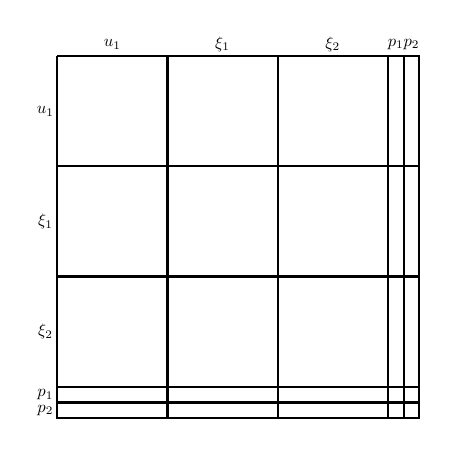
\begin{tikzpicture}[yscale=-1] 

\pgfmathsetmacro{\nt}{7};% time points
\pgfmathsetmacro{\nu}{1}; % controls
\pgfmathsetmacro{\nx}{2}; % states
\pgfmathsetmacro{\np}{2}; % parameters
\pgfmathsetmacro{\nc}{\nu + \nx}; % total continuous

%% control labels
\foreach \k in {1,...,\nu}{
	\pgfmathsetmacro{\x}{0.2*\nt*\k - 0.2/2*(\nt-1)};
	\node () at (\x,-0.05) {\scalebox{0.6}{$u_{\k}$}};
    \node () at (-0.05,\x) {\scalebox{0.6}{$u_{\k}$}};
}

%% state labels
\foreach \k in {1,...,\nx}{
	\pgfmathsetmacro{\x}{0.2*\nt*\k + 0.2*\nu*\nt - 0.2/2*(\nt-1)};
	\node () at (\x,-0.05) {\scalebox{0.6}{$\xi_{\k}$}};
    \node () at (-0.05,\x) {\scalebox{0.6}{$\xi_{\k}$}};
}

%% parameter labels
\foreach \k in {1,...,\np}{
	\pgfmathsetmacro{\x}{0.2*\k + 0.2*\nu*\nt + 0.2*\nx*\nt};
	\node () at (\x,-0.05) {\scalebox{0.6}{$p_{\k}$}};
    \node () at (-0.05,\x) {\scalebox{0.6}{$p_{\k}$}};
}


%% controls
\foreach \k in {1,...,\nu}{
	\foreach \j in {1,...,\nu}{
		\foreach \i in {1,...,\nt}{ 
        	\pgfmathsetmacro{\kk}{\k-1};
            \pgfmathsetmacro{\jj}{\j-1};
        	\pgfmathsetmacro{\x}{0.2*\i + 0.2*\kk*\nt};
            \pgfmathsetmacro{\y}{0.2*\i + 0.2*\jj*\nt};
        	\node () at (\x,\y) {\mysparsesymbol};
} 
    \pgfmathsetmacro{\kk}{\k-1};
    \pgfmathsetmacro{\jj}{\j-1};
    \pgfmathsetmacro{\x}{0.2*\kk*\nt + 0.1};
    \pgfmathsetmacro{\y}{0.2*\jj*\nt + 0.1};
	\draw[\mysparseboxcolor,thick](\x,\y) -- (\x+0.2*\nt,\y) -- (\x+0.2*\nt,\y+0.2*\nt) -- (\x,\y+0.2*\nt) -- (\x,\y);
} }

%% states
\foreach \k in {1,...,\nx}{
	\foreach \j in {1,...,\nx}{
		\foreach \i in {1,...,\nt}{ 
        	\pgfmathsetmacro{\kk}{\k-1};
            \pgfmathsetmacro{\jj}{\j-1};
        	\node () at (0.2*\i + 0.2*\kk*\nt + 0.2*\nu*\nt, 0.2*\i + 0.2*\jj*\nt + 0.2*\nu*\nt) {\mysparsesymbol};
} 
    \pgfmathsetmacro{\kk}{\k-1};
    \pgfmathsetmacro{\jj}{\j-1};
    \pgfmathsetmacro{\x}{0.2*\kk*\nt + 0.2*(\nu)*\nt + 0.1};
    \pgfmathsetmacro{\y}{0.2*\jj*\nt + 0.2*(\nu)*\nt + 0.1};
	\draw[\mysparseboxcolor,thick](\x,\y) -- (\x+0.2*\nt,\y) -- (\x+0.2*\nt,\y+0.2*\nt) -- (\x,\y+0.2*\nt) -- (\x,\y);
} }

%% parameters
\foreach \k in {1,...,\np}{
	\foreach \j in {1,...,\np}{
      \pgfmathsetmacro{\kk}{\k-1};
      \pgfmathsetmacro{\jj}{\j-1};
      \node ( ) at (0.2*\j + 0.2*\nx*\nt + 0.2*\nu*\nt, 0.2*\k + 0.2*\nx*\nt + 0.2*\nu*\nt) {\mysparsesymbol};
      \pgfmathsetmacro{\x}{0.2*\kk + 0.2*(\nu)*\nt + 0.2*\nx*\nt + 0.1};
      \pgfmathsetmacro{\y}{0.2*\jj + 0.2*(\nu)*\nt + 0.2*\nx*\nt + 0.1};
      \draw[\mysparseboxcolor,thick](\x,\y) -- (\x+0.2,\y) -- (\x+0.2,\y+0.2) -- (\x,\y+0.2) -- (\x,\y);
} }

%% states and controls
\foreach \k in {1,...,\nu}{
	\foreach \j in {1,...,\nx}{
		\foreach \i in {1,...,\nt}{ 
        	\pgfmathsetmacro{\kk}{\k-1};
            \pgfmathsetmacro{\jj}{\j-1};
        	\node () at ( 0.2*\i + 0.2*\kk*\nt , 0.2*\i + 0.2*\jj*\nt + 0.2*\nu*\nt) {\mysparsesymbol};
        	\node () at ( 0.2*\i + 0.2*\jj*\nt + 0.2*\nu*\nt, 0.2*\i + 0.2*\kk*\nt) {\mysparsesymbol};
} 
    \pgfmathsetmacro{\kk}{\k-1};
    \pgfmathsetmacro{\jj}{\j-1};
    \pgfmathsetmacro{\x}{0.2*\kk*\nt + 0.1};
    \pgfmathsetmacro{\y}{0.2*\jj*\nt + 0.2*(\nu)*\nt + 0.1};
	\draw[\mysparseboxcolor,thick](\x,\y) -- (\x+0.2*\nt,\y) -- (\x+0.2*\nt,\y+0.2*\nt) -- (\x,\y+0.2*\nt) -- (\x,\y);
    \draw[\mysparseboxcolor,thick](\y,\x) -- (\y+0.2*\nt,\x) -- (\y+0.2*\nt,\x+0.2*\nt) -- (\y,\x+0.2*\nt) -- (\y,\x);
} }

%% states and parameters
\foreach \k in {1,...,\np}{
	\foreach \j in {1,...,\nx}{
		\foreach \i in {1,...,\nt}{ 
        	\pgfmathsetmacro{\kk}{\k-1};
            \pgfmathsetmacro{\jj}{\j-1};
        	\node () at ( 0.2*\k + 0.2*\nx*\nt + 0.2*\nu*\nt, 0.2*\i + 0.2*\jj*\nt + 0.2*\nu*\nt ) {\mysparsesymbol};
            \node () at ( 0.2*\i + 0.2*\jj*\nt + 0.2*\nu*\nt, 0.2*\k + 0.2*\nx*\nt + 0.2*\nu*\nt ) {\mysparsesymbol};
} 
    \pgfmathsetmacro{\kk}{\k-1};
    \pgfmathsetmacro{\jj}{\j-1};
    \pgfmathsetmacro{\x}{0.2*\kk + 0.2*\nx*\nt + 0.2*\nu*\nt + 0.1};
    \pgfmathsetmacro{\y}{0.2*\jj*\nt + 0.2*\nu*\nt + 0.1};
	\draw[\mysparseboxcolor,thick](\x,\y) -- (\x+0.2,\y) -- (\x+0.2,\y+0.2*\nt) -- (\x,\y+0.2*\nt) -- (\x,\y);
    \draw[\mysparseboxcolor,thick](\y,\x) -- (\y+0.2*\nt,\x) -- (\y+0.2*\nt,\x+0.2) -- (\y,\x+0.2) -- (\y,\x);

} }

%% controls and parameters
\foreach \k in {1,...,\np}{
	\foreach \j in {1,...,\nu}{
		\foreach \i in {1,...,\nt}{ 
        	\pgfmathsetmacro{\kk}{\k-1};
            \pgfmathsetmacro{\jj}{\j-1};
        	\node () at ( 0.2*\k + 0.2*\nx*\nt + 0.2*\nu*\nt, 0.2*\i + 0.2*\jj*\nt ) {\mysparsesymbol};
            \node () at ( 0.2*\i + 0.2*\jj*\nt , 0.2*\k + 0.2*\nx*\nt + 0.2*\nu*\nt ) {\mysparsesymbol};
} 
    \pgfmathsetmacro{\kk}{\k-1};
    \pgfmathsetmacro{\jj}{\j-1};
    \pgfmathsetmacro{\x}{0.2*\kk + 0.2*\nx*\nt + 0.2*\nu*\nt + 0.1};
    \pgfmathsetmacro{\y}{0.2*\jj*\nt + 0.1};
	\draw[\mysparseboxcolor,thick](\x,\y) -- (\x+0.2,\y) -- (\x+0.2,\y+0.2*\nt) -- (\x,\y+0.2*\nt) -- (\x,\y);
    \draw[\mysparseboxcolor,thick](\y,\x) -- (\y+0.2*\nt,\x) -- (\y+0.2*\nt,\x+0.2) -- (\y,\x+0.2) -- (\y,\x);
} }

%% initial states
\foreach \k in {1,...,\nx}{
	\foreach \j in {1,...,\nc}{
		\foreach \i in {1,...,\nt}{ 
        	\pgfmathsetmacro{\kk}{\k-1};
            \pgfmathsetmacro{\jj}{\j-1};
        	\node () at (0.2 + 0.2*\kk*\nt + 0.2*\nu*\nt, 0.2*\i + 0.2*\jj*\nt ) {\mysparsesymbol};
            \node () at ( 0.2*\i + 0.2*\jj*\nt , 0.2 + 0.2*\kk*\nt + 0.2*\nu*\nt ) {\mysparsesymbol};
} } 
	\foreach \j in {1,...,\np}{
		\pgfmathsetmacro{\kk}{\k-1};
        \pgfmathsetmacro{\jj}{\j-1};
        \node () at ( 0.2*\k + 0.2*\nx*\nt + 0.2*\nu*\nt, 0.2 + 0.2*\jj*\nt + 0.2*\nu*\nt ) {\mysparsesymbol};
        \node () at ( 0.2 + 0.2*\jj*\nt + 0.2*\nu*\nt , 0.2*\k + 0.2*\nx*\nt + 0.2*\nu*\nt ) {\mysparsesymbol};
	}
}

%% final states
\foreach \k in {1,...,\nx}{
	\foreach \j in {1,...,\nc}{
		\foreach \i in {1,...,\nt}{ 
        	\pgfmathsetmacro{\kk}{\k-1};
            \pgfmathsetmacro{\jj}{\j-1};
        	\node () at (0.2*\nt + 0.2*\kk*\nt + 0.2*\nu*\nt, 0.2*\i + 0.2*\jj*\nt ) {\mysparsesymbol};
            \node () at ( 0.2*\i + 0.2*\jj*\nt , 0.2*\nt + 0.2*\kk*\nt + 0.2*\nu*\nt ) {\mysparsesymbol};
} } 
	\foreach \j in {1,...,\np}{
		\pgfmathsetmacro{\kk}{\k-1};
        \pgfmathsetmacro{\jj}{\j-1};
        \node () at ( 0.2*\k + 0.2*\nx*\nt + 0.2*\nu*\nt, 0.2*\nt + 0.2*\jj*\nt + 0.2*\nu*\nt ) {\mysparsesymbol};
        \node () at ( 0.2*\nt + 0.2*\jj*\nt + 0.2*\nu*\nt , 0.2*\k + 0.2*\nx*\nt + 0.2*\nu*\nt ) {\mysparsesymbol};
	}
}


























% %% states and controls
% \foreach \k in {0,...,2}{
% 	\foreach \j in {0,...,2}{
% 		\foreach \i in {1,...,5}{ 
%         	\node () at (0.2*\i + \k,0.2*\i + \j) {\mysparsesymbol};
% } } }

% %% parameters - right
% \foreach \k in {0,...,1}{
% 	\foreach \j in {0,...,2}{
% 		\foreach \i in {1,...,5}{
%         	\node ( ) at (0.2*\k + 3.2, 0.2*\i + \j) {\mysparsesymbol};
% } } }

% %% parameters - bottom
% \foreach \k in {0,...,1}{
% 	\foreach \j in {0,...,2}{
% 		\foreach \i in {1,...,5}{
%         	\node ( ) at (0.2*\i + \j, 0.2*\k + 3.2) {\mysparsesymbol};
% } } }

% %% parameters - corner
% \foreach \k in {0,...,1}{
% 	\foreach \j in {0,...,1}{
%         	\node ( ) at (0.2*\j + 3.2, 0.2*\k + 3.2) {\mysparsesymbol};
% } }

% %% initial states - bottom
% \foreach \k in {0,...,1}{
% 	\foreach \j in {0,...,2}{
% 		\foreach \i in {1,...,5}{
%         	\node ( ) at (0.2*\i + \j, \k + 1.2) {\mysparsesymbol};
% } } }

% %% final states - bottom
% \foreach \k in {0,...,1}{
% 	\foreach \j in {0,...,2}{
% 		\foreach \i in {1,...,5}{
%         	\node ( ) at (0.2*\i + \j, \k + 2.0) {\mysparsesymbol};
% } } }

% %% initial states - right
% \foreach \k in {0,...,1}{
% 	\foreach \j in {0,...,2}{
% 		\foreach \i in {1,...,5}{
%         	\node ( ) at (\k + 1.2, 0.2*\i + \j) {\mysparsesymbol};
% } } }

% %% final states - right
% \foreach \k in {0,...,1}{
% 	\foreach \j in {0,...,2}{
% 		\foreach \i in {1,...,5}{
%         	\node ( ) at (\k + 2.0, 0.2*\i + \j) {\mysparsesymbol};
% } } }


% %% draw boxes - states and controls
% \foreach \k in {0,...,2}{
% 	\foreach \j in {0,...,2}{
%     	\pgfmathsetmacro{\x}{\k + 0.1};
%     	\pgfmathsetmacro{\y}{\j + 0.1};
%         \draw[blue!70] (\x,\y) -- (\x+1,\y) -- (\x+1,\y+1) -- (\x,\y+1) -- (\x,\y);
% } }

% %% draw boxes - parameters - right
% \foreach \k in {0,...,1}{
% 	\foreach \j in {0,...,2}{
%     	\pgfmathsetmacro{\x}{0.2*\k + 0.1 + 3};
%     	\pgfmathsetmacro{\y}{\j + 0.1};
%         \draw[blue] (\x,\y) -- (\x+0.2,\y) -- (\x+0.2,\y+1) -- (\x,\y+1) -- (\x,\y);
% } }

% %% draw boxes - parameters - bottom
% \foreach \k in {0,...,2}{
% 	\foreach \j in {0,...,1}{
%     	\pgfmathsetmacro{\x}{\k + 0.1};
%     	\pgfmathsetmacro{\y}{0.2*\j + 0.1 + 3};
%         \draw[blue] (\x,\y) -- (\x+1,\y) -- (\x+1,\y+0.2) -- (\x,\y+0.2) -- (\x,\y);
% } }

% %% draw boxes - parameters - bottom
% \foreach \k in {0,...,1}{
% 	\foreach \j in {0,...,1}{
%     	\pgfmathsetmacro{\x}{0.2*\k + 0.1 + 3};
%     	\pgfmathsetmacro{\y}{0.2*\j + 0.1 + 3};
%         \draw[blue] (\x,\y) -- (\x+0.2,\y) -- (\x+0.2,\y+0.2) -- (\x,\y+0.2) -- (\x,\y);
% } }


%% final states
\foreach \k in {1,...,\nx}{
	\foreach \j in {1,...,\nc}{
		\foreach \i in {1,...,\nt}{ 
        	\pgfmathsetmacro{\kk}{\k-1};
            \pgfmathsetmacro{\jj}{\j-1};
        	\node () at (0.2*\nt + 0.2*\kk*\nt + 0.2*\nu*\nt, 0.2*\i + 0.2*\jj*\nt ) {\mytemp};
            \node () at ( 0.2*\i + 0.2*\jj*\nt , 0.2*\nt + 0.2*\kk*\nt + 0.2*\nu*\nt ) {\mytemp};
} } 
	\foreach \j in {1,...,\np}{
		\pgfmathsetmacro{\kk}{\k-1};
        \pgfmathsetmacro{\jj}{\j-1};
        \node () at ( 0.2*\k + 0.2*\nx*\nt + 0.2*\nu*\nt, 0.2*\nt + 0.2*\jj*\nt + 0.2*\nu*\nt ) {\mytemp};
        \node () at ( 0.2*\nt + 0.2*\jj*\nt + 0.2*\nu*\nt , 0.2*\k + 0.2*\nx*\nt + 0.2*\nu*\nt ) {\mytemp};
	}
}
\end{tikzpicture}
}
\vspace{-5mm}
\caption{$\bm{L}_{5j}$ and $\bm{L}_{i5}$ terms.}
\end{subfigure}
%%%%%%%%%%%
\begin{subfigure}[b]{0.45\textwidth}
\tikzsetnextfilename{Hoff}

\centering
\resizebox{1\textwidth}{!}{
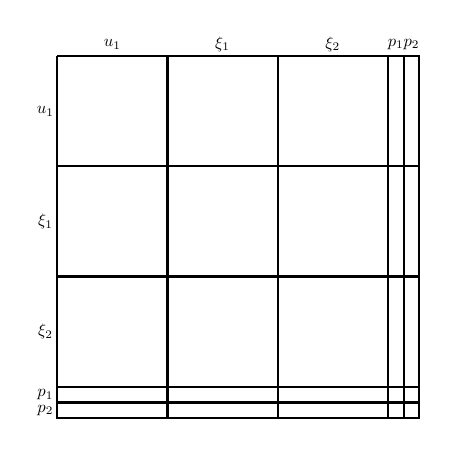
\begin{tikzpicture}[yscale=-1] 

\pgfmathsetmacro{\nt}{7};% time points
\pgfmathsetmacro{\nu}{1}; % controls
\pgfmathsetmacro{\nx}{2}; % states
\pgfmathsetmacro{\np}{2}; % parameters
\pgfmathsetmacro{\nc}{\nu + \nx}; % total continuous

%% control labels
\foreach \k in {1,...,\nu}{
	\pgfmathsetmacro{\x}{0.2*\nt*\k - 0.2/2*(\nt-1)};
	\node () at (\x,-0.05) {\scalebox{0.6}{$u_{\k}$}};
    \node () at (-0.05,\x) {\scalebox{0.6}{$u_{\k}$}};
}

%% state labels
\foreach \k in {1,...,\nx}{
	\pgfmathsetmacro{\x}{0.2*\nt*\k + 0.2*\nu*\nt - 0.2/2*(\nt-1)};
	\node () at (\x,-0.05) {\scalebox{0.6}{$\xi_{\k}$}};
    \node () at (-0.05,\x) {\scalebox{0.6}{$\xi_{\k}$}};
}

%% parameter labels
\foreach \k in {1,...,\np}{
	\pgfmathsetmacro{\x}{0.2*\k + 0.2*\nu*\nt + 0.2*\nx*\nt};
	\node () at (\x,-0.05) {\scalebox{0.6}{$p_{\k}$}};
    \node () at (-0.05,\x) {\scalebox{0.6}{$p_{\k}$}};
}


%% controls
\foreach \k in {1,...,\nu}{
	\foreach \j in {1,...,\nu}{
		\foreach \i in {1,...,\nt}{ 
        	\pgfmathsetmacro{\kk}{\k-1};
            \pgfmathsetmacro{\jj}{\j-1};
        	\pgfmathsetmacro{\x}{0.2*\i + 0.2*\kk*\nt};
            \pgfmathsetmacro{\y}{0.2*\i + 0.2*\jj*\nt};
        	\node () at (\x,\y) {\mysparsesymbol};
} 
    \pgfmathsetmacro{\kk}{\k-1};
    \pgfmathsetmacro{\jj}{\j-1};
    \pgfmathsetmacro{\x}{0.2*\kk*\nt + 0.1};
    \pgfmathsetmacro{\y}{0.2*\jj*\nt + 0.1};
	\draw[\mysparseboxcolor,thick](\x,\y) -- (\x+0.2*\nt,\y) -- (\x+0.2*\nt,\y+0.2*\nt) -- (\x,\y+0.2*\nt) -- (\x,\y);
} }

%% states
\foreach \k in {1,...,\nx}{
	\foreach \j in {1,...,\nx}{
		\foreach \i in {1,...,\nt}{ 
        	\pgfmathsetmacro{\kk}{\k-1};
            \pgfmathsetmacro{\jj}{\j-1};
        	\node () at (0.2*\i + 0.2*\kk*\nt + 0.2*\nu*\nt, 0.2*\i + 0.2*\jj*\nt + 0.2*\nu*\nt) {\mysparsesymbol};
} 
    \pgfmathsetmacro{\kk}{\k-1};
    \pgfmathsetmacro{\jj}{\j-1};
    \pgfmathsetmacro{\x}{0.2*\kk*\nt + 0.2*(\nu)*\nt + 0.1};
    \pgfmathsetmacro{\y}{0.2*\jj*\nt + 0.2*(\nu)*\nt + 0.1};
	\draw[\mysparseboxcolor,thick](\x,\y) -- (\x+0.2*\nt,\y) -- (\x+0.2*\nt,\y+0.2*\nt) -- (\x,\y+0.2*\nt) -- (\x,\y);
} }

%% parameters
\foreach \k in {1,...,\np}{
	\foreach \j in {1,...,\np}{
      \pgfmathsetmacro{\kk}{\k-1};
      \pgfmathsetmacro{\jj}{\j-1};
      \node ( ) at (0.2*\j + 0.2*\nx*\nt + 0.2*\nu*\nt, 0.2*\k + 0.2*\nx*\nt + 0.2*\nu*\nt) {\mysparsesymbol};
      \pgfmathsetmacro{\x}{0.2*\kk + 0.2*(\nu)*\nt + 0.2*\nx*\nt + 0.1};
      \pgfmathsetmacro{\y}{0.2*\jj + 0.2*(\nu)*\nt + 0.2*\nx*\nt + 0.1};
      \draw[\mysparseboxcolor,thick](\x,\y) -- (\x+0.2,\y) -- (\x+0.2,\y+0.2) -- (\x,\y+0.2) -- (\x,\y);
} }

%% states and controls
\foreach \k in {1,...,\nu}{
	\foreach \j in {1,...,\nx}{
		\foreach \i in {1,...,\nt}{ 
        	\pgfmathsetmacro{\kk}{\k-1};
            \pgfmathsetmacro{\jj}{\j-1};
        	\node () at ( 0.2*\i + 0.2*\kk*\nt , 0.2*\i + 0.2*\jj*\nt + 0.2*\nu*\nt) {\mysparsesymbol};
        	\node () at ( 0.2*\i + 0.2*\jj*\nt + 0.2*\nu*\nt, 0.2*\i + 0.2*\kk*\nt) {\mysparsesymbol};
} 
    \pgfmathsetmacro{\kk}{\k-1};
    \pgfmathsetmacro{\jj}{\j-1};
    \pgfmathsetmacro{\x}{0.2*\kk*\nt + 0.1};
    \pgfmathsetmacro{\y}{0.2*\jj*\nt + 0.2*(\nu)*\nt + 0.1};
	\draw[\mysparseboxcolor,thick](\x,\y) -- (\x+0.2*\nt,\y) -- (\x+0.2*\nt,\y+0.2*\nt) -- (\x,\y+0.2*\nt) -- (\x,\y);
    \draw[\mysparseboxcolor,thick](\y,\x) -- (\y+0.2*\nt,\x) -- (\y+0.2*\nt,\x+0.2*\nt) -- (\y,\x+0.2*\nt) -- (\y,\x);
} }

%% states and parameters
\foreach \k in {1,...,\np}{
	\foreach \j in {1,...,\nx}{
		\foreach \i in {1,...,\nt}{ 
        	\pgfmathsetmacro{\kk}{\k-1};
            \pgfmathsetmacro{\jj}{\j-1};
        	\node () at ( 0.2*\k + 0.2*\nx*\nt + 0.2*\nu*\nt, 0.2*\i + 0.2*\jj*\nt + 0.2*\nu*\nt ) {\mysparsesymbol};
            \node () at ( 0.2*\i + 0.2*\jj*\nt + 0.2*\nu*\nt, 0.2*\k + 0.2*\nx*\nt + 0.2*\nu*\nt ) {\mysparsesymbol};
} 
    \pgfmathsetmacro{\kk}{\k-1};
    \pgfmathsetmacro{\jj}{\j-1};
    \pgfmathsetmacro{\x}{0.2*\kk + 0.2*\nx*\nt + 0.2*\nu*\nt + 0.1};
    \pgfmathsetmacro{\y}{0.2*\jj*\nt + 0.2*\nu*\nt + 0.1};
	\draw[\mysparseboxcolor,thick](\x,\y) -- (\x+0.2,\y) -- (\x+0.2,\y+0.2*\nt) -- (\x,\y+0.2*\nt) -- (\x,\y);
    \draw[\mysparseboxcolor,thick](\y,\x) -- (\y+0.2*\nt,\x) -- (\y+0.2*\nt,\x+0.2) -- (\y,\x+0.2) -- (\y,\x);

} }

%% controls and parameters
\foreach \k in {1,...,\np}{
	\foreach \j in {1,...,\nu}{
		\foreach \i in {1,...,\nt}{ 
        	\pgfmathsetmacro{\kk}{\k-1};
            \pgfmathsetmacro{\jj}{\j-1};
        	\node () at ( 0.2*\k + 0.2*\nx*\nt + 0.2*\nu*\nt, 0.2*\i + 0.2*\jj*\nt ) {\mysparsesymbol};
            \node () at ( 0.2*\i + 0.2*\jj*\nt , 0.2*\k + 0.2*\nx*\nt + 0.2*\nu*\nt ) {\mysparsesymbol};
} 
    \pgfmathsetmacro{\kk}{\k-1};
    \pgfmathsetmacro{\jj}{\j-1};
    \pgfmathsetmacro{\x}{0.2*\kk + 0.2*\nx*\nt + 0.2*\nu*\nt + 0.1};
    \pgfmathsetmacro{\y}{0.2*\jj*\nt + 0.1};
	\draw[\mysparseboxcolor,thick](\x,\y) -- (\x+0.2,\y) -- (\x+0.2,\y+0.2*\nt) -- (\x,\y+0.2*\nt) -- (\x,\y);
    \draw[\mysparseboxcolor,thick](\y,\x) -- (\y+0.2*\nt,\x) -- (\y+0.2*\nt,\x+0.2) -- (\y,\x+0.2) -- (\y,\x);
} }

%% initial states
\foreach \k in {1,...,\nx}{
	\foreach \j in {1,...,\nc}{
		\foreach \i in {1,...,\nt}{ 
        	\pgfmathsetmacro{\kk}{\k-1};
            \pgfmathsetmacro{\jj}{\j-1};
        	\node () at (0.2 + 0.2*\kk*\nt + 0.2*\nu*\nt, 0.2*\i + 0.2*\jj*\nt ) {\mysparsesymbol};
            \node () at ( 0.2*\i + 0.2*\jj*\nt , 0.2 + 0.2*\kk*\nt + 0.2*\nu*\nt ) {\mysparsesymbol};
} } 
	\foreach \j in {1,...,\np}{
		\pgfmathsetmacro{\kk}{\k-1};
        \pgfmathsetmacro{\jj}{\j-1};
        \node () at ( 0.2*\k + 0.2*\nx*\nt + 0.2*\nu*\nt, 0.2 + 0.2*\jj*\nt + 0.2*\nu*\nt ) {\mysparsesymbol};
        \node () at ( 0.2 + 0.2*\jj*\nt + 0.2*\nu*\nt , 0.2*\k + 0.2*\nx*\nt + 0.2*\nu*\nt ) {\mysparsesymbol};
	}
}

%% final states
\foreach \k in {1,...,\nx}{
	\foreach \j in {1,...,\nc}{
		\foreach \i in {1,...,\nt}{ 
        	\pgfmathsetmacro{\kk}{\k-1};
            \pgfmathsetmacro{\jj}{\j-1};
        	\node () at (0.2*\nt + 0.2*\kk*\nt + 0.2*\nu*\nt, 0.2*\i + 0.2*\jj*\nt ) {\mysparsesymbol};
            \node () at ( 0.2*\i + 0.2*\jj*\nt , 0.2*\nt + 0.2*\kk*\nt + 0.2*\nu*\nt ) {\mysparsesymbol};
} } 
	\foreach \j in {1,...,\np}{
		\pgfmathsetmacro{\kk}{\k-1};
        \pgfmathsetmacro{\jj}{\j-1};
        \node () at ( 0.2*\k + 0.2*\nx*\nt + 0.2*\nu*\nt, 0.2*\nt + 0.2*\jj*\nt + 0.2*\nu*\nt ) {\mysparsesymbol};
        \node () at ( 0.2*\nt + 0.2*\jj*\nt + 0.2*\nu*\nt , 0.2*\k + 0.2*\nx*\nt + 0.2*\nu*\nt ) {\mysparsesymbol};
	}
}


























% %% states and controls
% \foreach \k in {0,...,2}{
% 	\foreach \j in {0,...,2}{
% 		\foreach \i in {1,...,5}{ 
%         	\node () at (0.2*\i + \k,0.2*\i + \j) {\mysparsesymbol};
% } } }

% %% parameters - right
% \foreach \k in {0,...,1}{
% 	\foreach \j in {0,...,2}{
% 		\foreach \i in {1,...,5}{
%         	\node ( ) at (0.2*\k + 3.2, 0.2*\i + \j) {\mysparsesymbol};
% } } }

% %% parameters - bottom
% \foreach \k in {0,...,1}{
% 	\foreach \j in {0,...,2}{
% 		\foreach \i in {1,...,5}{
%         	\node ( ) at (0.2*\i + \j, 0.2*\k + 3.2) {\mysparsesymbol};
% } } }

% %% parameters - corner
% \foreach \k in {0,...,1}{
% 	\foreach \j in {0,...,1}{
%         	\node ( ) at (0.2*\j + 3.2, 0.2*\k + 3.2) {\mysparsesymbol};
% } }

% %% initial states - bottom
% \foreach \k in {0,...,1}{
% 	\foreach \j in {0,...,2}{
% 		\foreach \i in {1,...,5}{
%         	\node ( ) at (0.2*\i + \j, \k + 1.2) {\mysparsesymbol};
% } } }

% %% final states - bottom
% \foreach \k in {0,...,1}{
% 	\foreach \j in {0,...,2}{
% 		\foreach \i in {1,...,5}{
%         	\node ( ) at (0.2*\i + \j, \k + 2.0) {\mysparsesymbol};
% } } }

% %% initial states - right
% \foreach \k in {0,...,1}{
% 	\foreach \j in {0,...,2}{
% 		\foreach \i in {1,...,5}{
%         	\node ( ) at (\k + 1.2, 0.2*\i + \j) {\mysparsesymbol};
% } } }

% %% final states - right
% \foreach \k in {0,...,1}{
% 	\foreach \j in {0,...,2}{
% 		\foreach \i in {1,...,5}{
%         	\node ( ) at (\k + 2.0, 0.2*\i + \j) {\mysparsesymbol};
% } } }


% %% draw boxes - states and controls
% \foreach \k in {0,...,2}{
% 	\foreach \j in {0,...,2}{
%     	\pgfmathsetmacro{\x}{\k + 0.1};
%     	\pgfmathsetmacro{\y}{\j + 0.1};
%         \draw[blue!70] (\x,\y) -- (\x+1,\y) -- (\x+1,\y+1) -- (\x,\y+1) -- (\x,\y);
% } }

% %% draw boxes - parameters - right
% \foreach \k in {0,...,1}{
% 	\foreach \j in {0,...,2}{
%     	\pgfmathsetmacro{\x}{0.2*\k + 0.1 + 3};
%     	\pgfmathsetmacro{\y}{\j + 0.1};
%         \draw[blue] (\x,\y) -- (\x+0.2,\y) -- (\x+0.2,\y+1) -- (\x,\y+1) -- (\x,\y);
% } }

% %% draw boxes - parameters - bottom
% \foreach \k in {0,...,2}{
% 	\foreach \j in {0,...,1}{
%     	\pgfmathsetmacro{\x}{\k + 0.1};
%     	\pgfmathsetmacro{\y}{0.2*\j + 0.1 + 3};
%         \draw[blue] (\x,\y) -- (\x+1,\y) -- (\x+1,\y+0.2) -- (\x,\y+0.2) -- (\x,\y);
% } }

% %% draw boxes - parameters - bottom
% \foreach \k in {0,...,1}{
% 	\foreach \j in {0,...,1}{
%     	\pgfmathsetmacro{\x}{0.2*\k + 0.1 + 3};
%     	\pgfmathsetmacro{\y}{0.2*\j + 0.1 + 3};
%         \draw[blue] (\x,\y) -- (\x+0.2,\y) -- (\x+0.2,\y+0.2) -- (\x,\y+0.2) -- (\x,\y);
% } }


%% states and controls
\foreach \k in {1,...,\nu}{
	\foreach \j in {1,...,\nx}{
		\foreach \i in {1,...,\nt}{ 
        	\pgfmathsetmacro{\kk}{\k-1};
            \pgfmathsetmacro{\jj}{\j-1};
        	\node () at ( 0.2*\i + 0.2*\kk*\nt , 0.2*\i + 0.2*\jj*\nt + 0.2*\nu*\nt) {\mytemp};
        	\node () at ( 0.2*\i + 0.2*\jj*\nt + 0.2*\nu*\nt, 0.2*\i + 0.2*\kk*\nt) {\mytemp};
} } }

%% states and parameters
\foreach \k in {1,...,\np}{
	\foreach \j in {1,...,\nx}{
		\foreach \i in {1,...,\nt}{ 
        	\pgfmathsetmacro{\kk}{\k-1};
            \pgfmathsetmacro{\jj}{\j-1};
        	\node () at ( 0.2*\k + 0.2*\nx*\nt + 0.2*\nu*\nt, 0.2*\i + 0.2*\jj*\nt + 0.2*\nu*\nt ) {\mytemp};
            \node () at ( 0.2*\i + 0.2*\jj*\nt + 0.2*\nu*\nt, 0.2*\k + 0.2*\nx*\nt + 0.2*\nu*\nt ) {\mytemp};
} } }

%% controls and parameters
\foreach \k in {1,...,\np}{
	\foreach \j in {1,...,\nu}{
		\foreach \i in {1,...,\nt}{ 
        	\pgfmathsetmacro{\kk}{\k-1};
            \pgfmathsetmacro{\jj}{\j-1};
        	\node () at ( 0.2*\k + 0.2*\nx*\nt + 0.2*\nu*\nt, 0.2*\i + 0.2*\jj*\nt ) {\mytemp};
            \node () at ( 0.2*\i + 0.2*\jj*\nt , 0.2*\k + 0.2*\nx*\nt + 0.2*\nu*\nt ) {\mytemp};
} } }

\end{tikzpicture}
}
\vspace{-5mm}
\caption{Remaining terms.}
\end{subfigure}

\caption{Sparsity pattern of $\mathcal{H}$ matrix for all considered methods except CQHS.\label{fig:figsparsityHSS}}
\end{figure}